\section{Use case}
\label{sec:use_case}
Gli \glossario{use case} sono uno strumento grafico che permette di analizzare e approfondire i \glossario{requisiti utente} per arrivare a definire i \glossario{requisiti software} del sistema.

\subsection{Visualizzazione dataset caricato}

\begin{figure}[H]
    \centering
    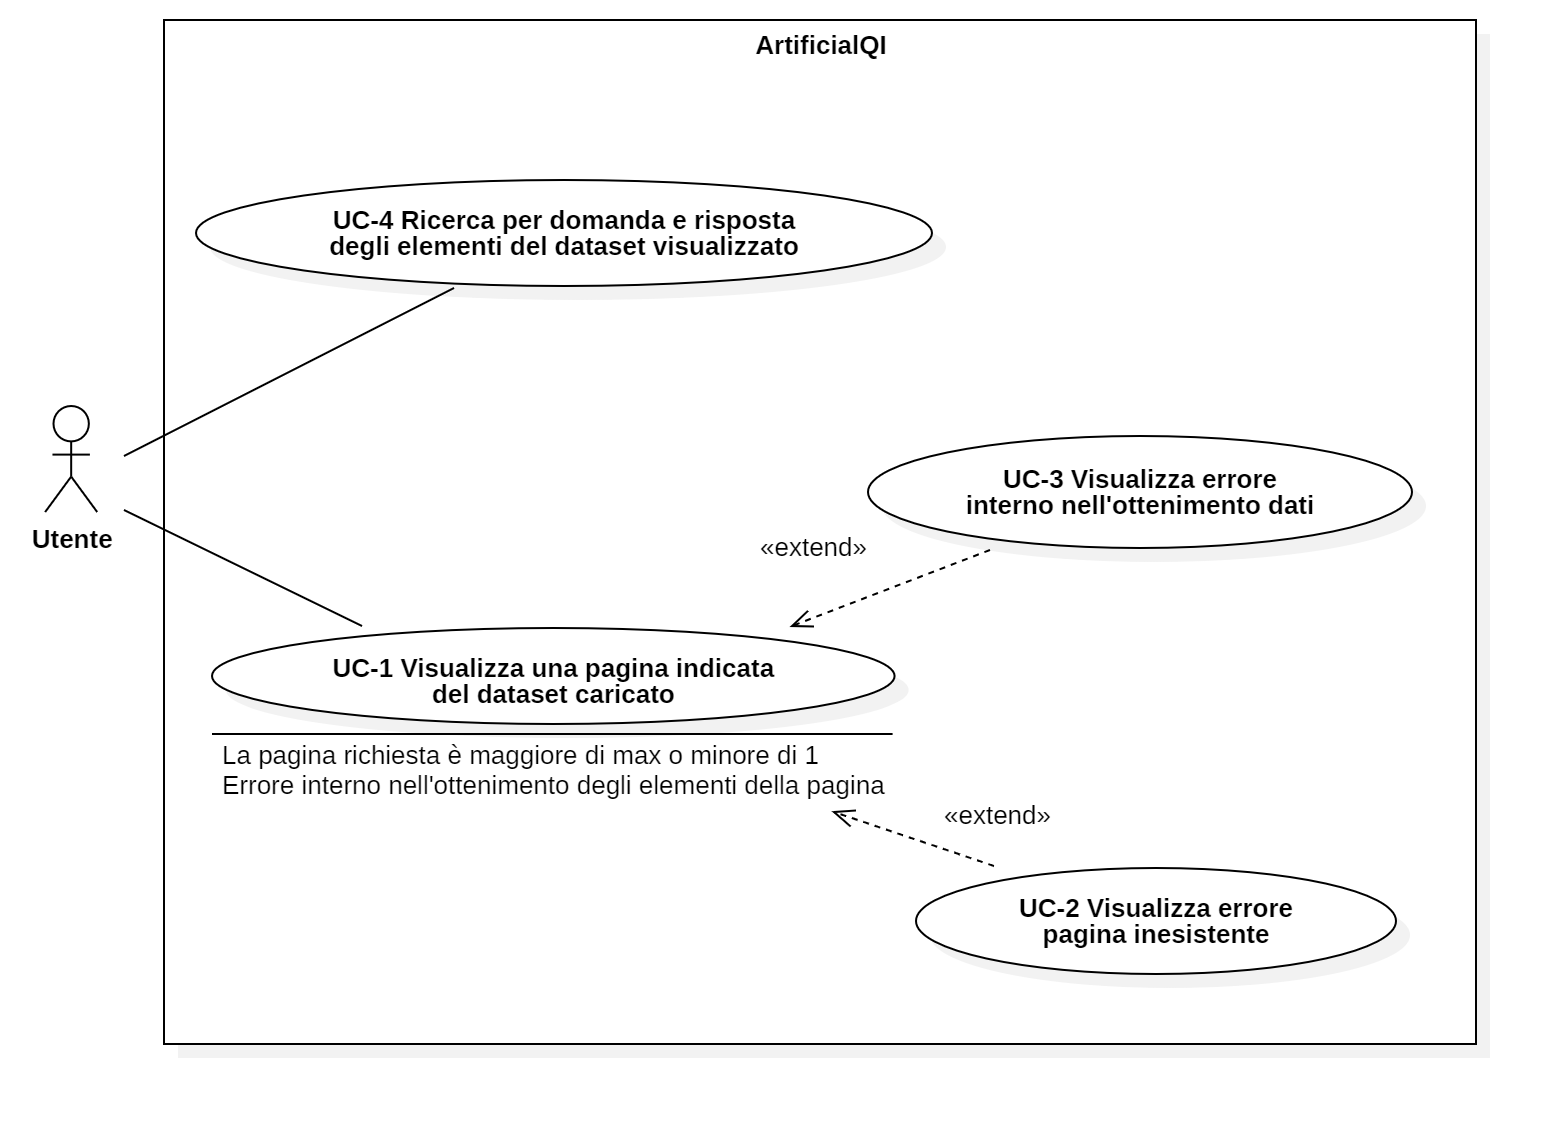
\includegraphics[scale=0.23]{Sezioni/UseCase/Immagini/VisualizzazioneDatasetCaricato}
    \caption{Diagramma visualizzazione dataset caricato.}
\end{figure}

\begin{usecase}{UC-1}{Visualizza il contenuto del dataset caricato}
    \label{uc:UC-1}    
    
    \req{\hyperref[ru:RUO-1]{RUO-1}} 

    \pre{
        \item L'utente ha caricato un dataset
    }

    \post{
        \item Viene visualizzata la prima pagina del dataset caricato
    }
    
    \actor{Utente}

    \subactors{}

    \trigger{L'utente vuole visualizzare il contenuto del dataset caricato}
    
    \inc{\hyperref[uc:UC-2]{UC-2}}

    \base{}

    \scenario{
        \item L'utente richiede la visualizzazione del contenuto del dataset caricato
        \item Viene visualizzata la prima pagina del dataset caricato o l'ultima pagina richiesta dall'utente secondo \hyperref[uc:UC-2]{UC-2}
    }

    \subscenario{
        \item[1.1] I'ultima versione del dataset caricato è vuoto:
        \begin{itemize}
            \item[a.] Viene indicato all'utente che il datataset caricato è vuoto
        \end{itemize}
    }
\end{usecase}


\begin{usecase}{UC-2}{Visualizza pagina dataset caricato}
    \label{uc:UC-2}
    
    \req{} 

    \pre{
        \item La pagina del dataset caricato da visualizzare esiste
    }

    \post{
        \item Viene visualizzato il contenuto della pagina del dataset caricato
    }
    
    \actor{Utente}

    \subactors{}

    \trigger{Il sistema deve visualizzare una pagina del dataset caricato}

    \inc{}

    \base{}

    
    \scenario{
        \item Il sistema ottiene gli elementi che compongono la pagina del dataset caricato
        \item Gli elementi vengono visualizzati in una lista
    }

    \subscenario{
        \item[1.1] Errore interno durante l'ottenimento degli elementi:
        \begin{itemize}
            \item[a.] \hyperref[uc:UC-3]{UC-3}
        \end{itemize}
    }

\end{usecase}

\begin{usecase}{UC-3}{Visualizza errore interno nell'ottenimento dati}
    \label{uc:UC-3}
    
    \req{} 

    \pre{
        \item Avviene un errore interno al sistema durante l'ottenimento di uno o più dati gestiti da esso    
    }

    \post{
        \item L'utente è a conoscenza dell'errore interno avvenuto
    }

    \actor{Utente}

    \subactors{}

    \trigger{Il sistema riscontra un errore interno durante l'ottenimento di dati}

    \inc{}

    \base{}

    \scenario{
        \item Viene mostrato un messaggio di errore che informa l'utente sulla natura dell'errore
    }

    \subscenario{}

\end{usecase}


\begin{usecase}{UC-4}{Cambia pagina del dataset visualizzato}
    \label{uc:UC-4}
    
    \req{\hyperref[ru:RUO-1]{RUO-1}} 

    \pre{
        \item L'utente sta visualizzando il dataset caricato \hyperref[uc:UC-1]{UC-1}
        \item Il dataset caricato non è vuoto
    }

    \post{
        \item L'utente visualizza la pagina del dataset caricato che ha richiesto
    }
    
    \actor{Utente}

    \subactors{}

    \trigger{L'utente vuole visualizzare una pagina del dataset caricato}
    
    \inc{\hyperref[uc:UC-2]{UC-2}}

    \base{}

    \scenario{
        \item L'utente richiede la visualizzazione di una precisa pagina del dataset caricato
        \item Il sistema controlla che la pagina richiesta esista
        \item Viene visualizzata la pagina richiesta secondo \hyperref[uc:UC-2]{UC-2} 
    }

    \subscenario{
        \item[2.1] La pagina richiesta non esiste ovvero è minore di uno o maggiore della pagina massima:
        \begin{itemize}
            \item[a.] \hyperref[uc:UC-5]{UC-5}
        \end{itemize}
    }

\end{usecase}

\begin{usecase}{UC-5}{Visualizza errore pagina inesistente}
    \label{uc:UC-5}
    
    \req{} 

    \pre{
        \item Il controllo di validità del numero di pagina fallisce
    }

    \post{
        \item L'utente capisce che la pagina richiesta non esiste e conosce il range di pagine valide
    }

    \actor{Utente}

    \subactors{}

    \trigger{Il sistema ha ricevuto una richiesta di visualizzazione per una pagina inesistente}

    \inc{}

    \base{}

    \scenario{
        \item Viene visualizzato un messaggio di errore che informa l'utente che la pagina richiesta non esiste
        \item Viene indicato il range di pagine valide 
    }

    \subscenario{}

\end{usecase}


\begin{usecase}{UC-6}{Ricerca per domanda e risposta degli elementi del dataset visualizzato}
    \label{uc:UC-6}
    
    \req{\hyperref[ru:RUO-2]{RUO-2}} 

    \pre{
        \item L'utente sta visualizzando il dataset caricato \hyperref[uc:UC-1]{UC-1}
    }

    \post{
        \item Il dataset caricato viene ristretto all'insieme di elementi risultanti dalla ricerca
        \item Il dataset caricato ristretto viene visualizzato
    }
    
    \actor{Utente}

    \subactors{}

    \trigger{L'utente vuole eseguire una ricerca per domanda e risposta sul dataset caricato}
    
    \inc{\hyperref[uc:UC-1]{UC-1}}

    \base{}

    \scenario{
        \item L'utente specifica le parole chiave da utilizzare nella ricerca
        \item Il sistema ricerca gli elementi che contengono le parole chiave nella propria domanda e/o risposta
        \item Il sistema restringe internamente il dataset caricato agli elementi risultanti dalla ricerca
        \item Viene visualizzato il dataset caricato ristretto secondo \hyperref[uc:UC-1]{UC-1}
    }

    \subscenario{}

\end{usecase}

\subsection{Modifica dataset visualizzato}

\begin{figure}[H]
    \centering
    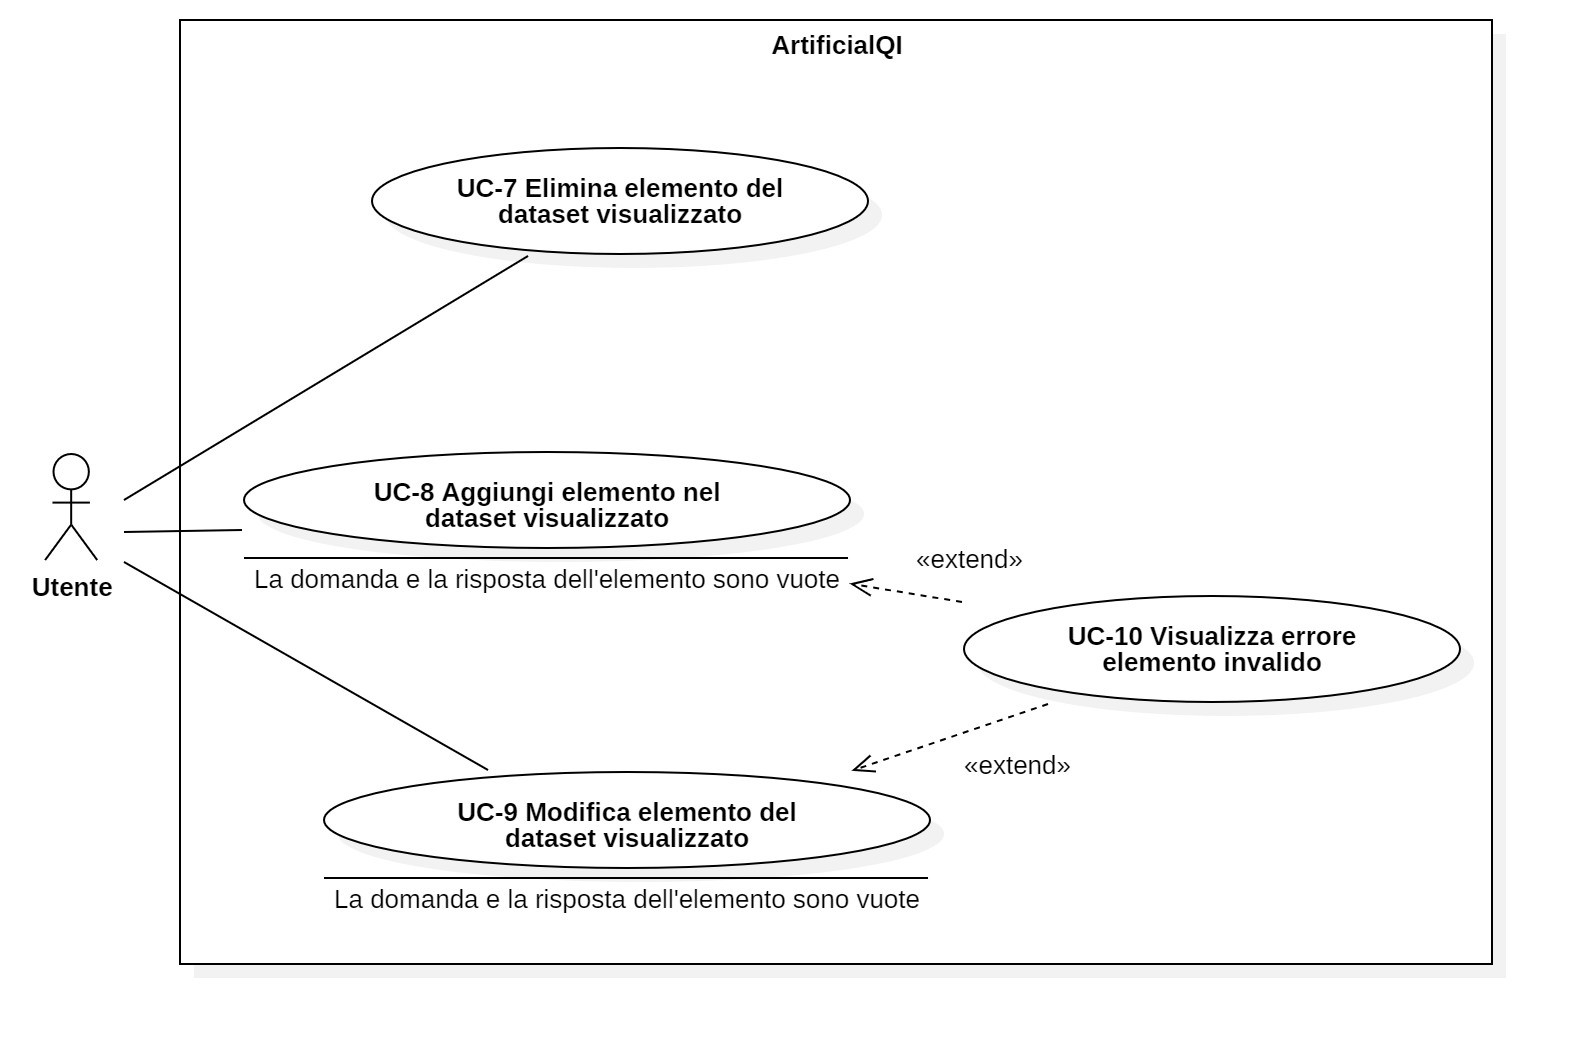
\includegraphics[scale=0.5]{Sezioni/UseCase/Immagini/ModificaDatasetVisualizzato.png}
    \caption{Diagramma modifica dataset visualizzato.}
\end{figure}



\begin{usecase}{UC-7}{Elimina elemento del dataset visualizzato}
    \label{uc:UC-7}
    
    \req{\hyperref[ru:RUO-1]{RUO-1}} 

    \pre{
        \item L'utente sta visualizzando la pagina del dataset caricato che contiene l'elemento da eliminare 
    }

    \post{
        \item L'elemento viene eliminato dal dataset visualizzato
    }
    
    \actor{Utente}

    \subactors{}

    \trigger{L'utente vuole eliminare un elemento contenuto nel dataset visualizzato}

    \inc{}

    \base{}

    \scenario{

        \item L'utente richiede l'eliminazione dell'elemento
        \item Il sistema richiede la conferma dell'eliminazione
        \item L'utente conferma l'eliminazione
        \item Il sistema elimina l'elemento dal dataset caricato
    }

    \subscenario{
        \item[3.1] L'utente annulla l'eliminazione:
        \begin{itemize}
            \item Il sistema annulla l'operazione
            \item Il sistema avvisa l'utente del corretto annullamento
        \end{itemize}
    }

\end{usecase}


\begin{usecase}{UC-8}{Aggiungi elemento nel dataset visualizzato}
    \label{uc:UC-8}
    
    \req{\hyperref[ru:RUO-1]{RUO-1}}

    \pre{
        \item L'utente sta visualizzando una pagina del dataset caricato \hyperref[uc:UC-1]{UC-1}
    }

    \post{
        \item L'elemento viene inserito nel dataset visualizzato
    }
    
    \actor{Utente}

    \subactors{}
    
    \trigger{L'utente vuole inserire un nuovo elemento nel dataset visualizzato}
    
    \inc{}

    \base{}

    \scenario{
        \item L'utente richiede l'inserimento di un nuovo elemento nel dataset visualizzato
        \item L'utente specifica la domanda e/o la risposta per il nuovo elemento
        \item L'utente conferma l'inserimento del nuovo elemento
        \item Il sistema verifica la correttezza dell'elemento
        \item Il sistema aggiunge l'elemento al dataset visualizzato
    }

    \subscenario{
        \item[3.1] L'utente annulla l'inserimento:
        \begin{itemize}
            \item Il sistema annulla l'operazione
        \end{itemize}
        \item[4.1] La domanda e la risposta sono vuote:
        \begin{itemize}
            \item \hyperref[uc:UC-10]{UC-10}
        \end{itemize}
    }

\end{usecase}

\begin{usecase}{UC-9}{Modifica elemento del dataset visualizzato}
    \label{uc:UC-9}
    
    \req{\hyperref[ru:RUO-1]{RUO-1}} 

    \pre{
        \item L'utente sta visualizzando la pagina del dataset caricato che contiene l'elemento da modificare 
    }

    \post{
        \item La modifica dell'elemento viene registrata nel dataset visualizzato
    }
    
    \actor{Utente}

    \subactors{}
    
    \trigger{L'utente vuole modificare un elemento del dataset visualizzato}
    
    \inc{}

    \base{}

    \scenario{
        \item L'utente richiede la modifica di un elemento
        \item L'utente modifica la domanda e/o la risposta dell'elemento
        \item L'utente conferma la modifica
        \item Il sistema verifica la correttezza della modifica
        \item Il sistema registra la modifica nel dataset visualizzato
    }

    \subscenario{
        \item[3.1] L'utente annulla l'inserimento:
        \begin{itemize}
            \item Il sistema annulla l'operazione
        \end{itemize}
        \item[4.1] La domanda e la risposta sono vuote:
        \begin{itemize}
            \item \hyperref[uc:UC-10]{UC-10}
        \end{itemize}
    }

\end{usecase}

\begin{usecase}{UC-10}{Visualizza errore elemento invalido}
    \label{uc:UC-10}
    
    \req{}

    \pre{
        \item Il sistema ha verificato la presenza di un elemento invalido
    }

    \post{
        \item L'utente viene avvisato e viene guidato nella corretta compilazione dell'elemento
    }
    
    \actor{Utente}

    \subactors{}

    \trigger{Domanda e riposta di un elemento sono entrambe vuote}
    
    \inc{}

    \base{}

    \scenario{
        \item Viene visualizzato un messaggio che spiega la presenza di un elemento invalido 
        \item Viene indicato come compilare correttamente un elemento
    }

    \subscenario{}

\end{usecase}




\subsection{Salvataggio dataset}

\begin{figure}[H]
    \centering
    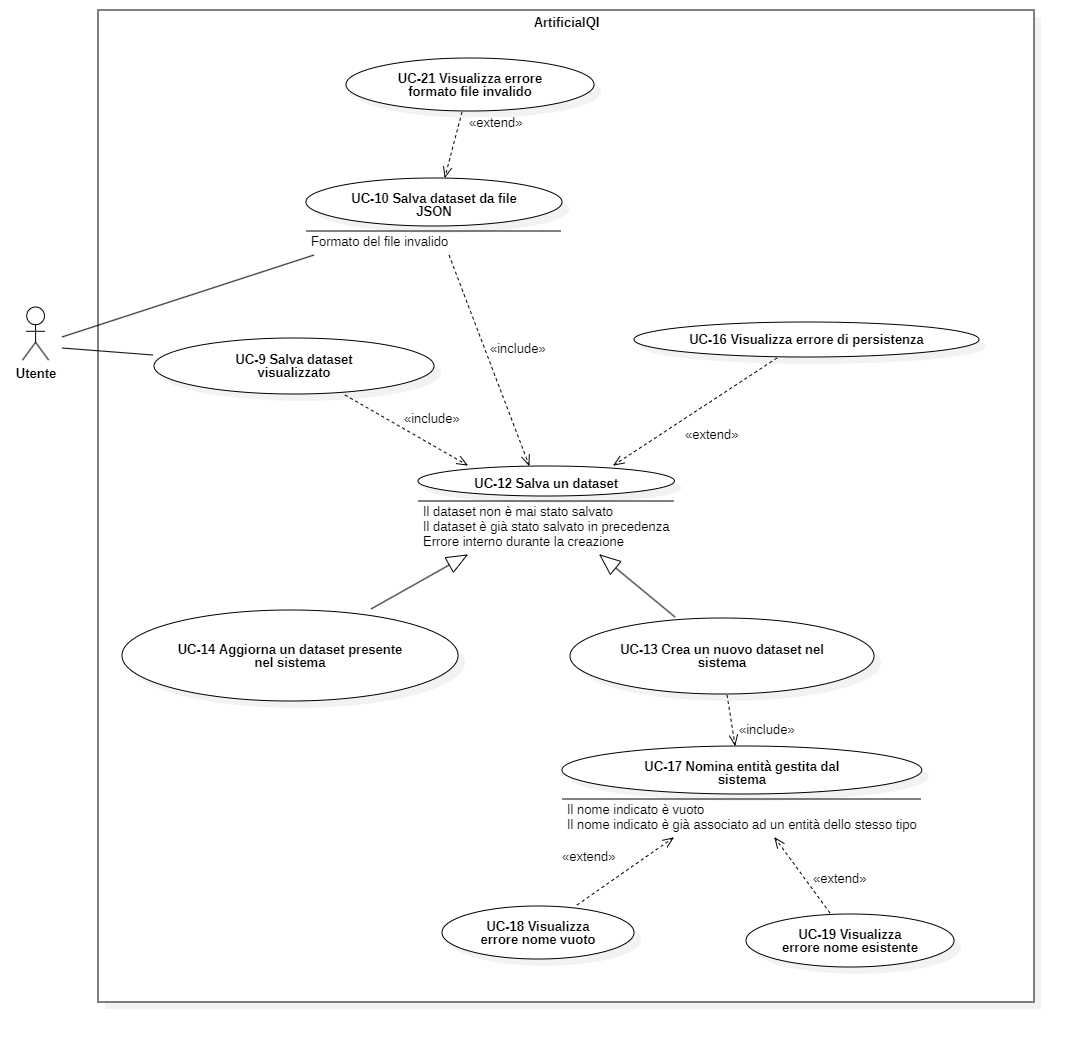
\includegraphics[scale=0.43]{Sezioni/UseCase/Immagini/SalvataggioDataset.png}
    \caption{Diagramma salvataggio dataset.}
\end{figure}

\begin{figure}[H]
    \label{fig:aggiornamento_dataset}
    \centering
    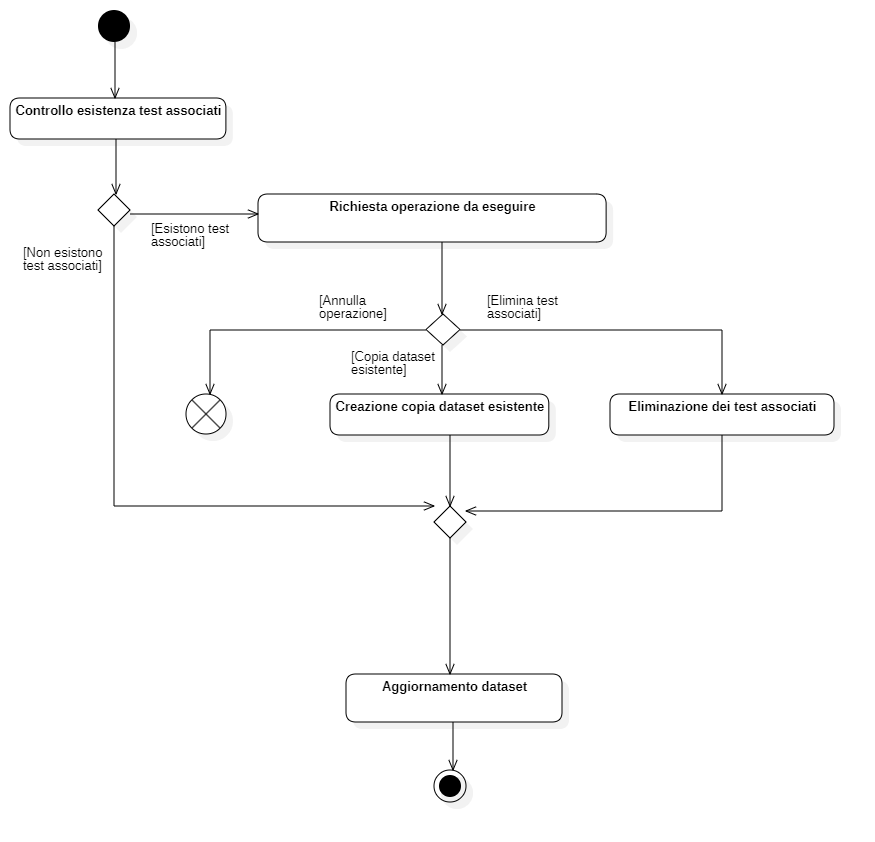
\includegraphics[scale=0.43]{Sezioni/UseCase/Immagini/AggiornamentoDataset_attivita.png}
    \caption{Diagramma aggiornamento dataset.}
\end{figure}


\begin{usecase}{UC-9}{Salva dataset visualizzato}
    \label{uc:UC-9}    
    
    \req{\hyperref[ru:RUO-3]{RUO-3}} 

    \pre{
        \item L'utente sta visualizzando una pagina del dataset da salvare \hyperref[uc:UC-1]{UC-1}
        \item Il dataset visualizzato non è vuoto
        \item Il dataset visualizzato non possiede una versione salvata o possiede una versione salvata non aggiornata
    }

    \post{
        \item Il dataset visualizzato viene salvato nel sistema
    }
    
    \actor{Utente}

    \subactors{}

    \trigger{L'utente vuole salvare il dataset visualizzato}
    
    \inc{\hyperref[uc:UC-10]{UC-10}}

    \base{}

    \scenario{
        \item L'utente richiede il salvataggio del dataset visualizzato
        \item Il sistema esegue il salvataggio seguendo \hyperref[uc:UC-10]{UC-10}
    }

    \subscenario{}
\end{usecase}

\begin{usecase}{UC-10}{Salva un dataset}
    \label{uc:UC-10}
    
    \req{}

    \pre{
        \item Il dataset ha delle modifiche da salvare
    }

    \post{
        \item Le modifiche vengono salvate
    }

    \actor{Utente}

    \subactors{}

    \trigger{Il sistema deve salvare un dataset}

    \inc{}

    \base{}

    \scenario{
        \item Il sistema verifica che il dataset da salvare sia stato già salvato in precedenza
    }
    
    \subscenario{
        \item [1.1] Errore interno durante la creazione:
        \begin{itemize}
            \item \hyperref[uc:UC-13]{UC-13}
        \end{itemize}
    }
\end{usecase}

\begin{usecase}{UC-11}{Creazione nuovo dataset nel sistema}
    \label{uc:UC-11}
    
    \req{} 

    \pre{
        \item Il dataset non è mai stato salvato
    }

    \post{
        \item Il dataset viene salvato 
    }
    
    \actor{Utente}

    \subactors{}

    \trigger{Il sistema deve salvare un nuovo dataset}

    \inc{\hyperref[uc:UC-14]{UC-14}}

    \base{\hyperref[uc:UC-10]{UC-10}}

    \scenario{
        \item Viene richiesta l'assegnazione di un nome per il nuovo dataset seguendo \hyperref[uc:UC-14]{UC-14}
        \item L'utente conferma la creazione di un nuovo dataset
        \item Il sistema salva il dataset
    }

    \subscenario{
        \item [1.1] L'utente annulla la creazione:
        \begin{itemize}
            \item Il sistema interrompe l'operazione
        \end{itemize}
    }

\end{usecase}

\begin{usecase}{UC-12}{Aggiorna dataset presente nel sistema}
    \label{uc:UC-12}
    
    \req{} 

    \pre{
        \item Il dataset è stato già salvato in precedenza 
    }

    \post{
        \item La versione del dataset salvata viene aggiornata
    }

    \actor{Utente}
    
    \subactors{}

    \trigger{Il sistema deve aggiornare la versione salvata di un dataset}

    \inc{}

    \base{\hyperref[uc:UC-10]{UC-10}}

    \scenario{
        \item Il sistema verifica la presenza di test associati alla versione del dataset da aggiornare
        \item Il sistema aggiorna la versione salvata seguendo \hyperref[fig:aggiornamento_dataset]{Aggiornamento dataset}
    }

    \subscenario{}

\end{usecase}

\begin{usecase}{UC-13}{Visualizza errore di persistenza}
    \label{uc:UC-13}
    
    \req{} 

    \pre{
        \item Il sistema riscontra un errore interno durante il salvataggio di uno o più dati
    }

    \post{
        \item L'utente conosce l'errore avvenuto
    }
    
    \actor{Utente}

    \subactors{}

    \trigger{Il sistema riscontra un errore interno durante il salvataggio}
    
    \inc{}

    \base{}

    \scenario{
        \item Viene visualizzato un messaggio di errore che spiega la natura dell'errore stesso
    }

    \subscenario{}

\end{usecase}


\begin{usecase}{UC-14}{Nomina entità gestita dal sistema}
    \label{uc:UC-14}
    
    \req{} 

    \pre{
        \item Il sistema deve ottenere dall'utente un nome da associare a un entità(dataset, esecuzione test o LLM)
    }

    \post{
        \item Il sistema possiede un nome valido per l'entità
    }
    
    \actor{Utente}

    \subactors{}

    \trigger{L'utente deve assegnare un nome a un entità gestita dal sistema}
    
    \inc{}

    \base{}

    \scenario{
        \item l'utente specifica il nome
        \item Il sistema verifica che il nome non sia vuoto
        \item Il sistema verifica che il nome non sia già associato a un altra entità dello stesso tipo
    }

    \subscenario{
        \item[2.1] Il nome è vuoto:
        \begin{itemize}
            \item \hyperref[uc:UC-15]{UC-15}
        \end{itemize}
        \item[3.1] Il nome esiste già:
        \begin{itemize}
            \item \hyperref[uc:UC-16]{UC-16}
        \end{itemize}

    }

\end{usecase}

\begin{usecase}{UC-15}{Visualizza errore nome vuoto}
    \label{uc:UC-15}
    
    \req{} 

    \pre{
        \item Il nome immesso dall'utente è vuoto 
    }

    \post{
        \item L'utente capisce che il nome vuoto non è valido 
    }

    \actor{Utente}

    \subactors{}

    \trigger{L'utente ha indicato un nome per un'entità che è vuoto}

    \inc{}

    \base{}

    \scenario{
        \item Viene visualizzato un messaggio di errore che informa l'utente che non è possibile utilizzare un nome vuoto
    }

    \subscenario{}

\end{usecase}

\begin{usecase}{UC-16}{Visualizza errore nome esistente}
    \label{uc:UC-16}
    
    \req{} 

    \pre{
        \item Il nome immesso dall'utente è già presente nel sistema
    }

    \post{
        \item L'utente capisce che il nome indicato non è disponibile 
    }

    \actor{Utente}

    \subactors{}

    \trigger{L'utente ha indicato un nome per un entità che è già associato a un entità dello stesso tipo}

    \inc{}

    \base{}

    \scenario{
        \item Viene visualizzato un messaggio di errore che informa l'utente che il nome indicato non è disponibile
    }

    \subscenario{}

\end{usecase}

\begin{usecase}{UC-17}{Salva dataset da file JSON}
    \label{uc:UC-17}
    
    \req{\hyperref[ru:RUF-4]{RUF-4}} 

    \pre{
        \item L'utente sta visualizzando i dataset salvati \hyperref[uc:UC-18]{UC-18}
    }

    \post{
        \item Viene salvato un nuovo dataset costruito a partire dal contenuto del file JSON selezionato dall'utente
    }

    \actor{Utente}

    \subactors{}

    \trigger{L'utente vuole salvare un nuovo dataset a partire da un file JSON}

    \inc{\hyperref[uc:UC-11]{UC-11}}

    \base{}

    \scenario{
        \item L'utente richiede il salvataggio di un nuovo dataset a partire da un file JSON
        \item L'utente seleziona il file JSON
        \item Il sistema verifica la validità del file caricato
        \item Il sistema salva un nuovo dataset usando il file JSON caricato seguendo \hyperref[uc:UC-11]{UC-11}
    }

    \subscenario{
        \item[2.1] Il file caricato non rispetta il formato atteso:
        \begin{itemize}
            \item \hyperref[uc:UC-18]{UC-18}
        \end{itemize}
    }

\end{usecase}

\begin{usecase}{UC-18}{Visualizza errore formato file invalido}
    \label{uc:UC-18}
    
    \req{}

    \pre{
        \item Il sistema ha ricevuto un file in un formato invalido 
    }

    \post{
        \item l'utente conosce il formato atteso
    }

    \actor{Utente}

    \subactors{}

    \trigger{L'utente fornisce un file in un formato invalido}

    \inc{}

    \base{}

    \scenario{
        \item Il sistema visualizza un messaggio di errore
        \item Il sistema visualizza un esempio del formato atteso
    }

    \subscenario{}

\end{usecase}





\subsection{Visualizzazione dataset salvati}

\begin{figure}[H]
    \centering
    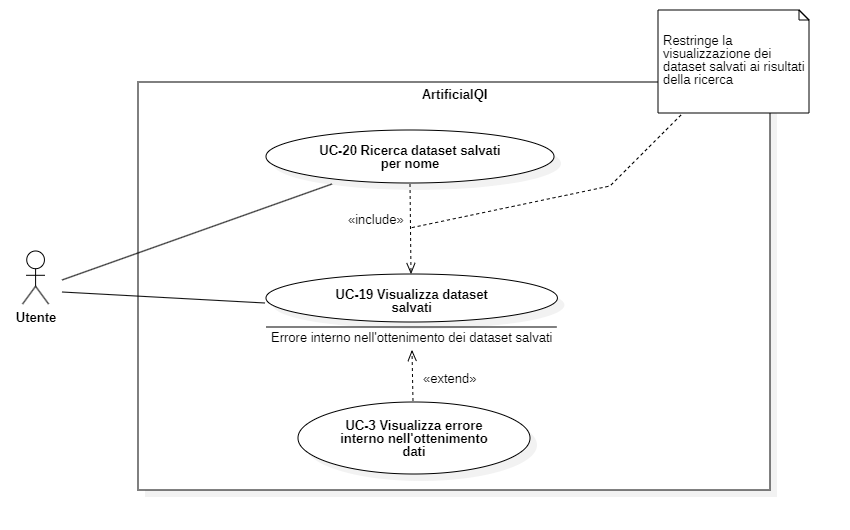
\includegraphics[scale=0.47]{Sezioni/UseCase/Immagini/VisualizzazioneDatasetSalvati}
    \caption{Diagramma visualizzazione dataset salvati.}
\end{figure}

\begin{usecase}{UC-22}{Visualizza dataset salvati}
    \label{uc:UC-22}
    
    \req{\hyperref[ru:RUO-3]{RUO-3}} 

    \pre{}

    \post{
        \item L'utente visualizza i dataset salvati
    }
    
    \actor{Utente}

    \trigger{L'utente vuole visualizzare i dataset salvati}

    \inc{}

    \base{}

    \scenario{
        \item L'utente richiede di visualizzare i dataset salvati
        \item Il sistema ottiene i dataset salvati
        \item Il sistema verifica la presenza di dataset salvati
        \item Vengono visualizzata la lista dei dataset salvati
    }

    \subscenario{
        \item[2.1] Il sistema verifica un errore interno durante l'ottenimento dei dataset salvati:
        \begin{itemize}
            \item \hyperref[uc:UC-3]{UC-3}
        \end{itemize}
        \item[3.1] Non esistono dataset salvati:
        \begin{itemize}
            \item Viene notificato all'utente che non esistono dataset salvati
        \end{itemize}
    }
\end{usecase}


\begin{usecase}{UC-23}{Ricerca dataset salvati per nome}
    \label{uc:UC-23}
    
    \req{\hyperref[ru:RUO-4]{RUO-4}} 

    \pre{
        \item L'utente sta visualizzando i dataset salvati
    }

    \post{
        \item L'utente visualizza la lista dei dataset salvati che contengono nel nome le parole chiave indicate
    }
    
    \actor{Utente}

    \trigger{L'utente richiede l'esecuzione della ricerca}

    \inc{\hyperref[uc:UC-22]{UC-22}}

    \base{}

    \scenario{
        \item L'utente specifica le parole chiave da utilizzare nella ricerca
        \item L'utente richiede l'esecuzione della ricerca
        \item Il sistema seleziona l'insieme di dataset salvati che contengono le parole chiave nel nome
        \item Il sistema mostra il precedente insieme seguendo \hyperref[uc:UC-22]{UC-22}
    }
    \subscenario{}
\end{usecase}


\subsection{Modifica dataset salvati}

\begin{figure}[H]
    \centering
    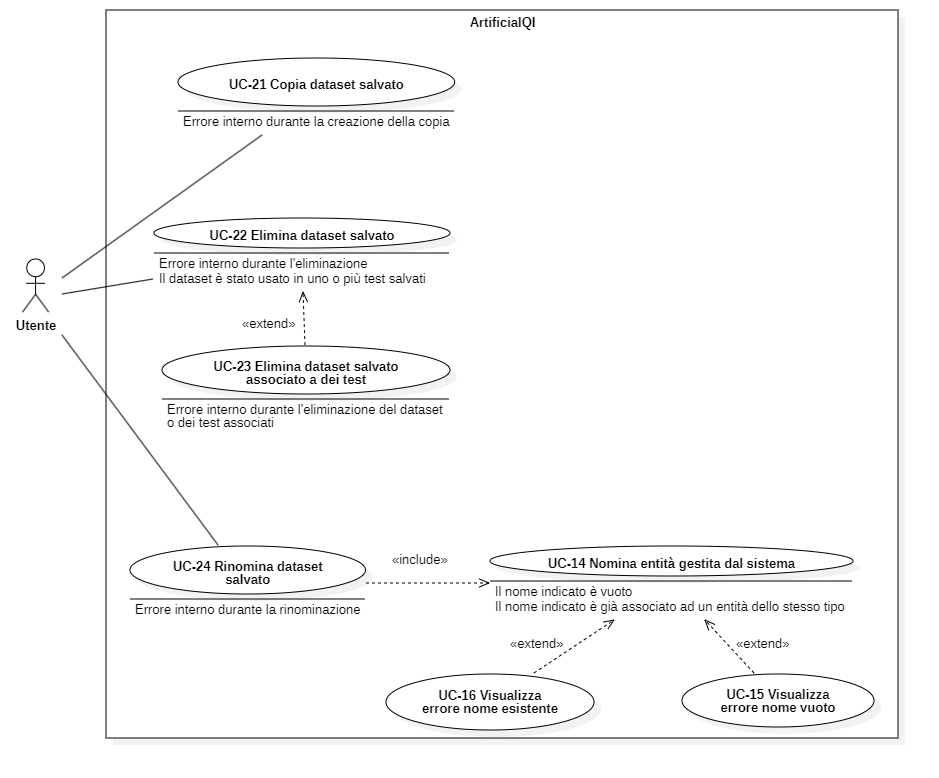
\includegraphics[scale=0.2]{Sezioni/UseCase/Immagini/ModificaDatasetSalvato.png}
    \caption{Diagramma modifica dataset salvati.}
\end{figure}

\begin{usecase}{UC-24}{Copia dataset salvato}
    \label{uc:UC-24}
    
    \req{\hyperref[ru:RUO-3]{RUO-3}} 

    \pre{
        \item L'utente sta visualizzando i dataset salvati \hyperref[uc:UC-22]{UC-22}
    }

    \post{
        \item Il sistema crea una copia del dataset salvato
    }
    
    \actor{Utente}

    \subactors{}

    \trigger{L'utente vuole creare una copia di un dataset salvato}

    \inc{}

    \base{}

    \scenario{
        \item L'utente richiede di copiare un dataset salvato
        \item Il sistema crea una copia del dataset salvato avente nome predefinito
        \item Il sistema notifica l'utente che la copia è andata a buon fine
    }

    \subscenario{
        \item[2.1] Avviene un errore interno al sistema durante la creazione della copia:
        \begin{itemize}
            \item \hyperref[uc:UC-16]{UC-16}
        \end{itemize}
    }
\end{usecase}


\begin{usecase}{UC-25}{Elimina dataset salvato}
    \label{uc:UC-25}
    
    \req{\hyperref[ru:RUO-3]{RUO-3}} 

    \pre{
        \item L'utente sta visualizzando i dataset salvati
    }

    \post{
        \item Il sistema elimina il dataset salvato che è quindi irrecuperabile
    }
    
    \actor{Utente}

    \subactors{}

    \trigger{L'utente richiede l'eliminazione di un dataset salvato}

    \inc{}

    \base{}

    \scenario{
        \item L'utente specifica il dataset salvato da eliminare
        \item Il sistema verifica che non esistano test che hanno utilizzato una qualsiasi versione del dataset
        \item Il sistema richiede la conferma dell'eliminazione
        \item L'utente conferma l'eliminazione
        \item Il sistema elimina il dataset salvato
        \item Il sistema avvisa l'utente della corretta eliminazione
    }
    \subscenario{
        \item[2.1] Il dataset da eliminare è stato usato nella sua versione attuale o nelle precedenti in uno o più test salvati:
        \begin{itemize}
            \item \hyperref[uc:UC-26]{UC-26}
        \end{itemize}
        \item[4.1] L'utente annulla l'operazione di eliminazione:
        \begin{itemize}
            \item Il sistema annulla l'operazione
            \item Lo stato del sistema resta invariato
            \item L'utente viene notificato del corretto annullamento
        \end{itemize} 
        \item[5.1] Avviene un errore interno al sistema durante l'eliminazione:
        \begin{itemize}
            \item \hyperref[uc:UC-16]{UC-16}
        \end{itemize}
    }
\end{usecase}

\begin{usecase}{UC-26}{Elimina dataset salvato associato a dei test}
    \label{uc:UC-26}
    
    \req{} 

    \pre{
        \item Il dataset da eliminare è associato a uno o più test
    }

    \post{
        \item Il dataset e i test a esso associati vengono eliminati e sono quindi irrecuperabili
    }
    
    \actor{}

    \subactors{}

    \trigger{Il sistema deve eliminare un dataset associato a uno o più test}

    \inc{}

    \base{}

    \scenario{
        \item Il sistema visualizza la lista di test associati al dataset e avvisa l'utente che verranno eliminati
        \item L'utente conferma l'eliminazione
        \item Il sistema elimina il dataset 
        \item Il sistema elimina i test associati
        \item Il sistema avvisa l'utente della corretta eliminazione
    }
    \subscenario{
        \item[2.1] L'utente annulla l'operazione di eliminazione:
        \begin{itemize}
            \item Il sistema annulla l'operazione
            \item Lo stato del sistema resta invariato
            \item L'utente viene notificato del corretto annullamento
        \end{itemize} 
        \item[3.1] Avviene un errore interno al sistema durante l'eliminazione del dataset:
        \begin{itemize}
            \item \hyperref[uc:UC-16]{UC-16}
        \end{itemize}
        \item[4.1] Avviene un errore interno al sistema durante l'eliminazione dei test associati:
        \begin{itemize}
            \item \hyperref[uc:UC-16]{UC-16}
        \end{itemize}
    }
\end{usecase}

\begin{usecase}{UC-27}{Rinomina dataset salvato}
    \label{uc:UC-27}
    
    \req{\hyperref[ru:RUO-3]{RUO-3}} 

    \pre{
        \item L'utente sta visualizzando i dataset salvati \hyperref[uc:UC-22]{UC-22}
    }

    \post{
        \item Il sistema rinomina il dataset salvato indicato
    }
    
    \actor{Utente}

    \subactors{}

    \trigger{L'utente vuole rinominare un dataset salvato}

    \inc{\hyperref[uc:UC-17]{UC-17}}

    \base{}

    \scenario{
        \item L'utente richiede di rinominare un dataset salvato
        \item Il sistema ottiene il nuovo nome seguendo \hyperref[uc:UC-17]{UC-17}
        \item L'utente conferma la rinominazione
        \item Il sistema rinomina il dataset salvato
    }

    \subscenario{
        \item[3.1] L'utente annulla la rinominazione:
        \begin{itemize}
            \item Il sistema interrompe l'operazione
        \end{itemize}
        
        \item[4.1] Avviene un errore interno al sistema durante la rinominazione:
        \begin{itemize}
            \item \hyperref[uc:UC-16]{UC-16}
        \end{itemize}
        
    }
\end{usecase}



\subsection{Cambio dataset caricato}

\begin{figure}[H]
    \centering
    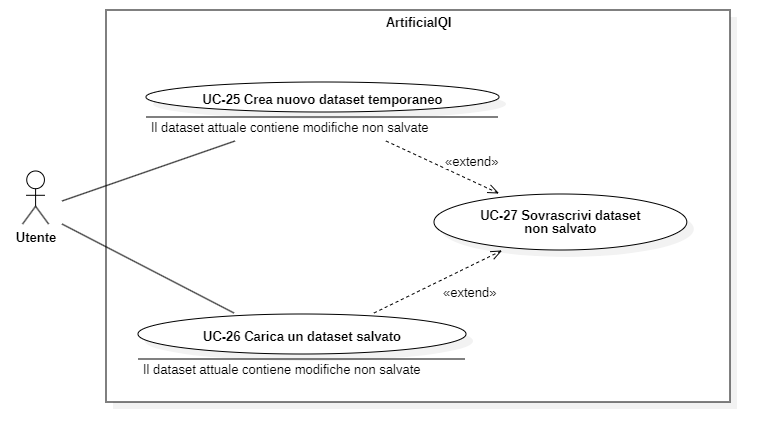
\includegraphics[scale=0.5]{Sezioni/UseCase/Immagini/CambioDatasetCaricato.png}
    \caption{Diagramma cambio dataset caricato.}
\end{figure}

\begin{usecase}{UC-28}{Crea nuovo dataset temporaneo}
    \label{uc:UC-28}
    
    \req{\hyperref[ru:RUO-3]{RUO-3}} 

    \pre{
        \item L'utente sta visualizzando la lista dei dataset salvati
    }

    \post{
        \item Il sistema carica un nuovo dataset vuoto
    }
    
    \actor{Utente}

    \subactors{}

    \trigger{L'utente vuole creare un nuovo dataset temporaneo}

    \inc{}

    \base{}

    \scenario{
        \item L'utente richiede la creazione di un nuovo dataset
        \item Il sistema verifica che il dataset attualmente caricato non abbia modifiche non salvate
        \item Il sistema carica un nuovo dataset vuoto temporaneo
    }

    \subscenario{
        \item[2.1] Il dataset caricato contiene modifiche non salvate:
        \begin{itemize}
            \item \hyperref[uc:UC-30]{UC-30}
        \end{itemize}
    }
\end{usecase}

\begin{usecase}{UC-29}{Carica un dataset salvato}
    \label{uc:UC-29}
    
    \req{\hyperref[ru:RUO-6]{RUO-6}} 

    \pre{
        \item L'utente sta visualizzando la lista dei dataset salvati
    }

    \post{
        \item Viene caricato il dataset salvato indicato
    }
    
    \actor{Utente}

    \subactors{}

    \trigger{L'utente richiede il caricamento di un dataset salvato}

    \inc{}

    \base{}

    \scenario{
        \item L'utente richiede il caricamento di un dataset salvato
        \item Il sistema verifica che il dataset attualmente caricato non abbia modifiche non salvate
        \item Il sistema carica il dataset salvato indicato
    }

    \subscenario{
        \item[2.1] Il dataset caricato contiene modifiche non salvate:
        \begin{itemize}
            \item \hyperref[uc:UC-30]{UC-30}
        \end{itemize}
    }
\end{usecase}

\begin{usecase}{UC-30}{Sovrascrivi dataset caricato}
    \label{uc:UC-30}
    
    \req{} 

    \pre{
        \item Esiste un dataset con modifiche non salvate
    }

    \post{
        \item Il dataset attuale viene sovrascritto dal dataset caricato e le modifiche non salvate vengono perse
    }
    
    \actor{Utente}

    \subactors{}

    \trigger{Il dataset attuale contiene delle modifiche non salvate e il sistema deve caricarne un altro}

    \inc{}

    \base{}

    \scenario{
        \item Il sistema richiede all'utente la conferma della sovrascrittura
        \item L'utente conferma la sovrascrittura
        \item Il sistema sovrascrive il dataset attuale con il dataset caricato 
    }

    \subscenario{
        \item[2.1] L'utente annulla la sovrascrittura:
        \begin{itemize}
            \item Il sistema interrompe l'operazione di caricamento
            \item Il dataset attuale resta invariato
        \end{itemize}
    }
\end{usecase}


\subsection{Esecuzione test}

\begin{figure}[H]
    \centering
    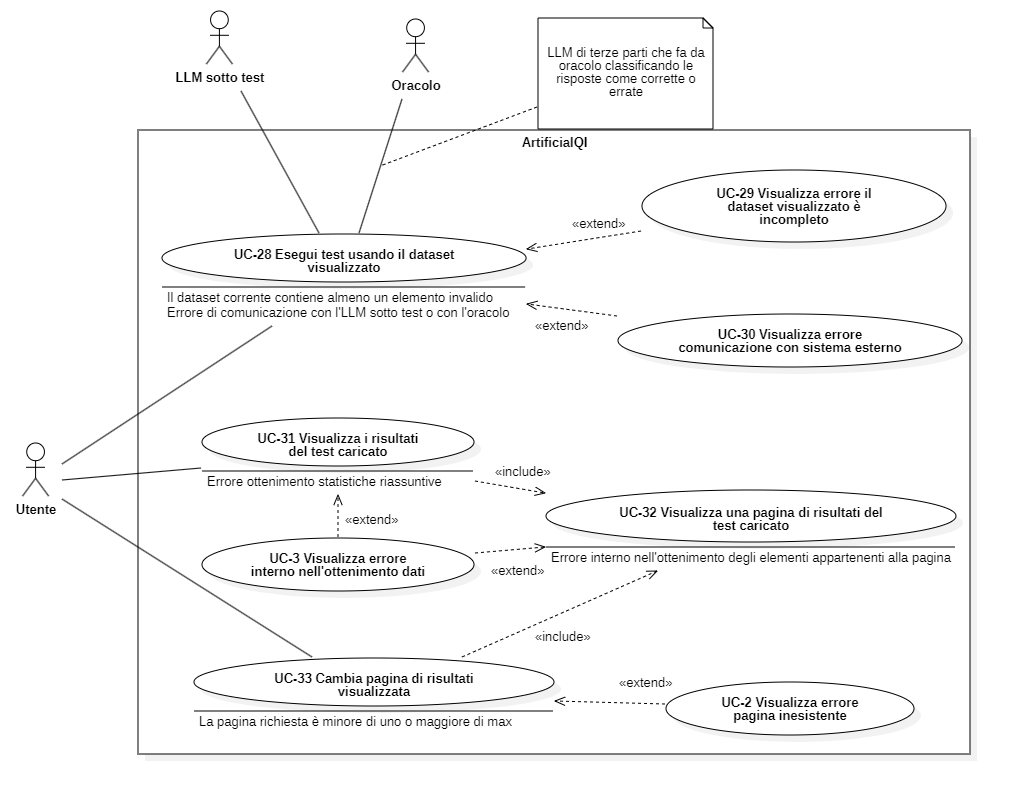
\includegraphics[scale=0.2]{Sezioni/UseCase/Immagini/EsecuzioneTest.png}
    \caption{Diagramma esecuzione test.}
\end{figure}

\begin{usecase}{UC-31}{Esegui test usando il dataset visualizzato}
    \label{uc:UC-31}
    
    \req{\hyperref[ru:RUO-7]{RUO-7}} 

    \pre{
        \item L'utente sta visualizzando il dataset da utilizzare per il test \hyperref[uc:UC-1]{UC-1}
        \item Il dataset visualizzato non è vuoto
    }

    \post{
        \item L'utente visualizza i risultati del test
    }
    
    \actor{Utente}

    \subactors{LLM sotto test, Oracolo}

    \trigger{L'utente vuole eseguire il test usando il dataset visualizzato}

    \inc{}

    \base{}

    \scenario{
        \item L'utente richiede di eseguire il test 
        \item L'utente seleziona un LLM da testare tra quelli salvati nel sistema
        \item Il sistema ottiene le risposte date dal LLM sotto test alle domande contenute nel dataset 
        \item Il sistema chiede all'oracolo la correttezza delle risposte
        \item Il sistema elabora i risultati del test
        \item I risultati del test vengono caricati come correnti
    }

    \subscenario{
        \item[1.1] Il dataset visualizzato contiene almeno un elemento incompleto ovvero con domanda o risposta vuote:
        \begin{itemize}
            \item \hyperref[uc:UC-32]{UC-32}
        \end{itemize}
        \item[2.1] Il sistema riscontra un errore di comunicazione con l'LLM sotto test:
        \begin{itemize}
            \item \hyperref[uc:UC-33]{UC-33}
        \end{itemize}
        \item[3.1] Il sistema riscontra un errore di comunicazione con l'oracolo:
        \begin{itemize}
            \item \hyperref[uc:UC-33]{UC-33}
        \end{itemize}
    }
\end{usecase}

\begin{usecase}{UC-32}{Visualizza errore dataset visualizzato è incompelto}
    \label{uc:UC-32}
    
    \req{} 

    \pre{
        \item Il dataset visualizzato contiene uno o più elementi con domanda o risposta vuote
    }

    \post{
        \item L'utente ottiene dei link alle pagine del dataset che contengono gli elementi incompleti
    }
    
    \actor{Utente}

    \trigger{Il sistema prima di eseguire il test individua elementi incompleti nel dataset}

    \inc{}

    \base{}

    \scenario{
        \item Viene visualizzata una lista di link alle pagine del dataset che contengono gli elementi incompleti evidenziati
    }

    \subscenario{}
\end{usecase}

\begin{usecase}{UC-33}{Visualizza errore di comunicazione con sistemma esterno}
    \label{uc:UC-33}
    
    \req{} 

    \pre{
        \item Il sistema interroga un sistema esterno e la comunicazione termina in modo anomalo
    }

    \post{
        \item L'utente viene messo al corrente dell'errore di comunicazione
    }
    
    \actor{Attore}

    \trigger{Il sistema riscontra un errore di comunicazione con un sistema esterno}

    \inc{}

    \base{}

    \scenario{
        \item Viene visualizzato un errore che specifica l'errore di comunicazione
    }

    \subscenario{}
\end{usecase}

\begin{usecase}{UC-34}{Visualizza i risultati del test caricato}
    \label{uc:UC-34}
    
    \req{\hyperref[ru:RUO-8]{RUO-8}} 

    \pre{
        \item Il test di cui si vuole visualizzare i risultati è stato caricato
    }

    \post{
        \item Vengono visualizzati i risultati del test caricato
    }
    
    \actor{Utente}

    \trigger{L'utente vuole visualizzare i risultati del test caricato}

    \inc{\hyperref[uc:UC-35]{UC-35}}

    \base{}

    \scenario{
        \item L'utente richiede la visualizzazione dei risultati del test caricato
        \item Viene visualizzata una dashboard contenente le statistiche sui risultati del test
        \item Viene visualizzata la prima pagina dei risultati del test seguendo \hyperref[uc:UC-35]{UC-35}
    }

    \subscenario{
        \item[2.1] Il sistema riscontra un errore durante l'ottenimento delle statistiche sui risultati del test:
        \begin{itemize}
            \item \hyperref[uc:UC-3]{UC-3}
        \end{itemize}
    }
\end{usecase}


\begin{usecase}{UC-35}{Visualizza pagina di risultati del test caricato}
    \label{uc:UC-35}
    
    \req{} 

    \pre{}

    \post{
        \item Viene visualizzata la pagina dei risultati del test caricato richiesta
    }
    
    \actor{Utente}

    \subactors{}

    \trigger{Il sistema deve visualizzare una precisa pagina dei risultati del test caricato}

    \inc{}

    \base{}

    \scenario{
        \item Il sistema ottiene i risultati del test per la pagina richiesta
        \item Il sistema mostra un diagramma di dispersione che rappresenta i singoli risultati della pagina sotto forma di punti 
        \item Viene visualizzata la lista dei singoli risultati appartenenti alla pagina richiesta
    }

    \subscenario{
        \item[1.1] Il sistema riscontra un errore interno durante l'ottenimento dei risultati appartenenti alla pagina da visualizzare:
        \begin{itemize}
            \item \hyperref[uc:UC-3]{UC-3}
        \end{itemize}
    }
\end{usecase}


\begin{usecase}{UC-36}{Cambia pagina di risultati visualizzata}
    \label{uc:UC-36}
    
    \req{} 

    \pre{
        \item L'utente sta visualizzando i risultati del test caricato
    }

    \post{
        \item Viene visualizzata la pagina dei risultati del test caricato richiesta
    }
    
    \actor{Utente}

    \subactors{}

    \trigger{L'utente vuole visualizzare una pagina dei risultati del test caricato}

    \inc{\hyperref[uc:UC-35]{UC-35}}

    \base{}

    \scenario{
        \item L'utente richiede la visualizzazione di una pagina di risultati del test
        \item Il sistema verifica che la pagina esista
        \item Il sistema visualizza la pagina richiesta seguendo \hyperref[uc:UC-35]{UC-35}
    }

    \subscenario{
        \item[2.1] La pagina richiesta è invalida ovvero minore di uno o maggiore della pagina massima:
        \begin{itemize}
            \item \hyperref[uc:UC-5]{UC-5}
        \end{itemize}
    }
\end{usecase}

\subsection{Visualizzazione di un elemento del diagramma di dispersione}

\begin{figure}[H]
    \centering
    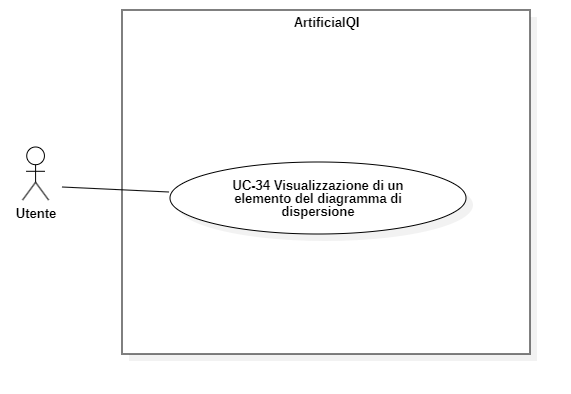
\includegraphics[scale=0.6]{Sezioni/UseCase/Immagini/InterazioneDiagrammaDispersione}
    \caption{Diagramma per la visualizzazione di un elemento del diagramma di dispersione.}
\end{figure}

\begin{usecase}{UC-34}{Visualizzazione di un elemento del diagramma di dispersione}
    \label{uc:UC-34}    
    
    \req{} 

    \pre{
        \item L'utente sta visualizzando i risultati del test caricato o sta visualizzando il confronto tra i singoli risultati di due test confrontati
    }

    \post{
        \item L'utente viene riportato al risultato relativo al risultato rappresentato dal punto del diagramma coinvolto nell'interazione 
    }
    
    \actor{Utente}

    \subactors{}

    \trigger{L'utente vuole visualizzare un elemento della pagina dei risultati del test}
    
    \inc{}

    \base{}

    \scenario{
        \item L'utente interagisce con un punto del diagramma di dispersione
        \item Il sistema rimanda l'utente al risultato che il punto rappresenta
    }

    \subscenario{}
\end{usecase}


\subsection{Salvataggio test}

\begin{figure}[H]
    \centering
    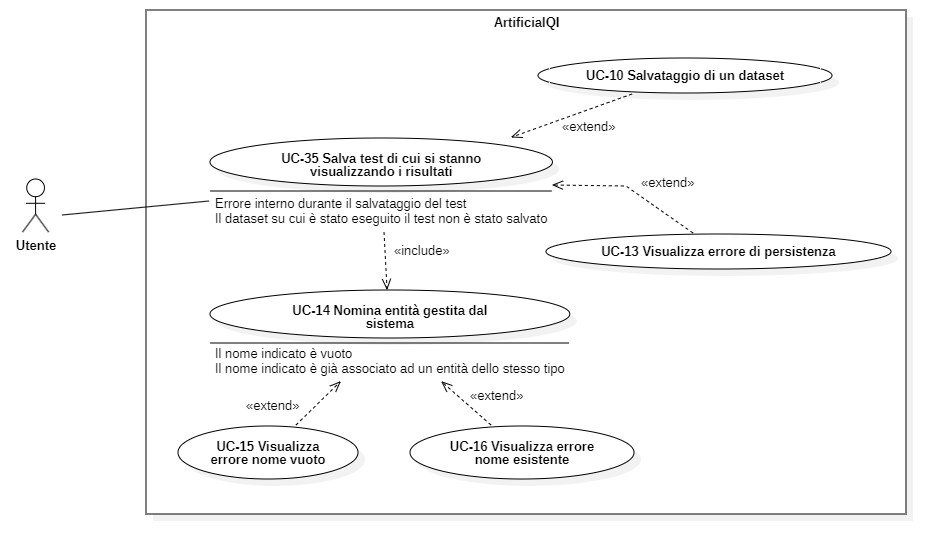
\includegraphics[scale=0.2]{Sezioni/UseCase/Immagini/SalvataggioTest.png}
    \caption{Salvataggio test.}
\end{figure}

\begin{usecase}{UC-38}{Salva test di cui si stanno visualizzando i risultati}
    \label{uc:UC-38}
    
    \req{RUF-1} 

    \pre{
        \item L'utente sta visualizzando i risultati del test da salvare
        \item Il test è sono ancora stato salvato nel sistema
    }

    \post{
        \item I risultati del test vengono salvati nel sistema
    }
    
    \actor{Utente}

    \subactors{}

    \trigger{L'utente vuole salvare i risultati del test}

    \inc{\hyperref[uc:UC-17]{UC-17}}

    \base{}

    \scenario{
        \item L'utente richiede di salvare il test
        \item Il sistema ottiene il nome per il nuovo test seguendo \hyperref[uc:UC-17]{UC-17}
        \item Il sistema verifica che il dataset su cui è stato eseguito il test è già stato salvato
        \item Il sistema salva il test 
        \item Il sistema notifica l'utente del corretto salvataggio
    }

    \subscenario{
        \item[3.1] Il dataset su cui è stato eseguito il test non è stato salvato:
        \begin{itemize}
            \item \hyperref[uc:UC-12]{UC-12}
        \end{itemize}
        \item[4.1] Il sistema verifica un errore interno durante il salvataggio del test:
        \begin{itemize}
            \item \hyperref[uc:UC-16]{UC-16}
        \end{itemize}
    }
\end{usecase}



\subsection{Visualizzazione test salvati}

\begin{figure}[H]
    \centering
    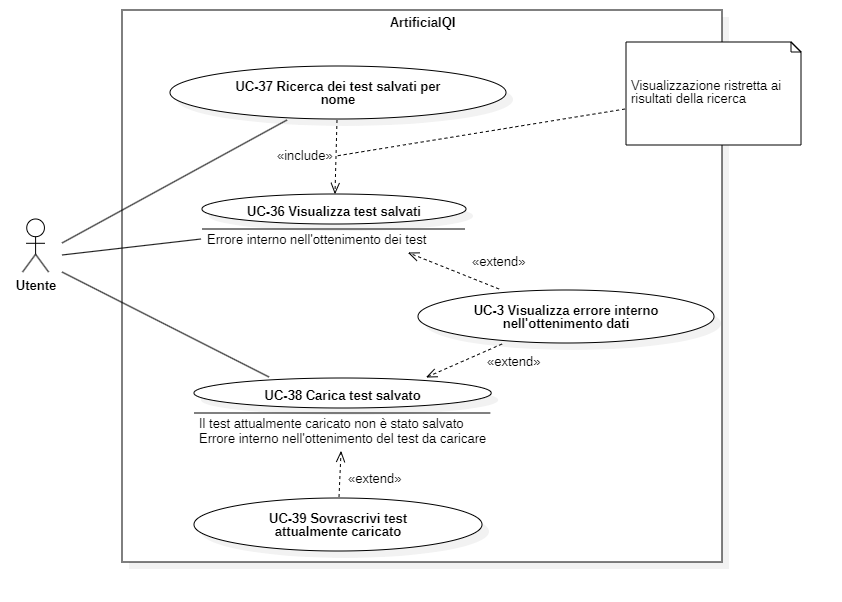
\includegraphics[scale=0.25]{Sezioni/UseCase/Immagini/VisualizzazioneTestSalvati}
    \caption{Diagramma per la visualizzazione di test salvati.}
\end{figure}

\begin{usecase}{UC-39}{Visualizza test salvati}
    \label{uc:UC-39}
    
    \req{\hyperref[ru:RUF-1]{RUF-1}}
    
    \pre{}
    
    \post{
        \item L'utente visualizza le esecuzioni di test salvate
    }
    
    \actor{
        Utente
    }
    
    \subactors{}
    
    \trigger{L'utente vuole visualizzare i test salvati}
    
    \inc{}
    
    \base{}
    
    \scenario{
        \item L'utente richiede la visualizzazione dei test salvati
        \item Il sistema ottiene i test salvati
        \item Il sistema visualizza i test salvati sotto forma di una lista
    }
    
    \subscenario{
        \item[2.1] Non esistono test salvati:
        \begin{itemize}
            \item Il sistema indica all'utente che non esistono test salvati
        \end{itemize}
        \item[2.2] Il sistema verifica un errore interno durante l'ottenimento dei test salvati:
        \begin{itemize}
            \item \hyperref[uc:UC-3]{UC-3}
        \end{itemize}
    }

\end{usecase}

\begin{usecase}{UC-40}{Ricerca dei test salvati per nome}
    \label{uc:UC-40}
    
    \req{\hyperref[ru:RUF-2]{RUF-2}}
    
    \pre{
        \item L'utente sta visualizzando i test salvati
    }
    
    \post{
        \item L'utente visualizza l'insieme di test salvati risultanti dalla ricerca
    }
    
    \actor{
        Utente
    }
    
    \subactors{}
    
    \trigger{L'utente vuole visualizzare i test salvati}
    
    \inc{\hyperref[uc:UC-39]{UC-39}}
    
    \base{}
    
    \scenario{
        \item L'utente indica le parole chiave da usare nella ricerca
        \item L'utente richiede l'esecuzione della ricerca
        \item Il sistema restringe i test salvati all'insieme di test che contengono nel proprio nome le parole chiave
        \item L'insieme di test ristretto viene visualizzato seguendo \hyperref[uc:UC-39]{UC-39}
    }
    
    \subscenario{}
\end{usecase}

\begin{usecase}{UC-41}{Carica test salvato}
    \label{uc:UC-41}
    
    \req{\hyperref[ru:RUF-3]{RUF-3}}
    
    \pre{
        \item L'utente sta visualizzando i test salvati
    }
    
    \post{
        \item Il test indicato dall'utente viene caricato nel sistema
    }
    
    \actor{
        Utente
    }
    
    \subactors{}
    
    \trigger{L'utente vuole caricare un test salvato}
    
    \inc{}
    
    \base{}
    
    \scenario{
        \item L'utente richiede il caricamento di un test visualizzato
        \item Il sistema verifica che il test attualmente caricato sia stato salvato
        \item Il sistema carica il test indicato
    }
    
    \subscenario{
        \item[2.1] Esiste un test attualmente caricato che non è stato salvato:
        \begin{itemize}
            \item \hyperref[uc:UC-42]{UC-42}
        \end{itemize}
        \item[2.2] Avviene un errore interno durante l'ottenimento del test indicato:
        \begin{itemize}
            \item \hyperref[uc:UC-3]{UC-3}
        \end{itemize}
    }
\end{usecase}

\begin{usecase}{UC-42}{Sovrascrivi test attualmente caricato}
    \label{uc:UC-42}
    
    \req{}
    
    \pre{
        \item Esiste un test caricato che non è ancora stato salvato
    }
    
    \post{
        \item Il test indicato dall'utente viene caricato nel sistema
    }
    
    \actor{Utente}
    
    \subactors{}
    
    \trigger{Il sistema deve caricare un test e quello attualmente caricato non è ancora stato salvato nel sistema}
    
    \inc{}
    
    \base{}
    
    \scenario{
        \item Il sistema richiede la conferma della sovrascrittura
        \item Il sistema procede con la sovrascrittura del test caricato che viene perso
    }
    
    \subscenario{
        \item[1.1] L'utente annulla la sovrascrittura:
        \begin{itemize}
            \item L'operazione di sovrascrittura termina
            \item Il test caricato resta invariato
        \end{itemize}
    }
\end{usecase}

\subsection{Modifica test salvato}

\begin{figure}[H]
    \centering
    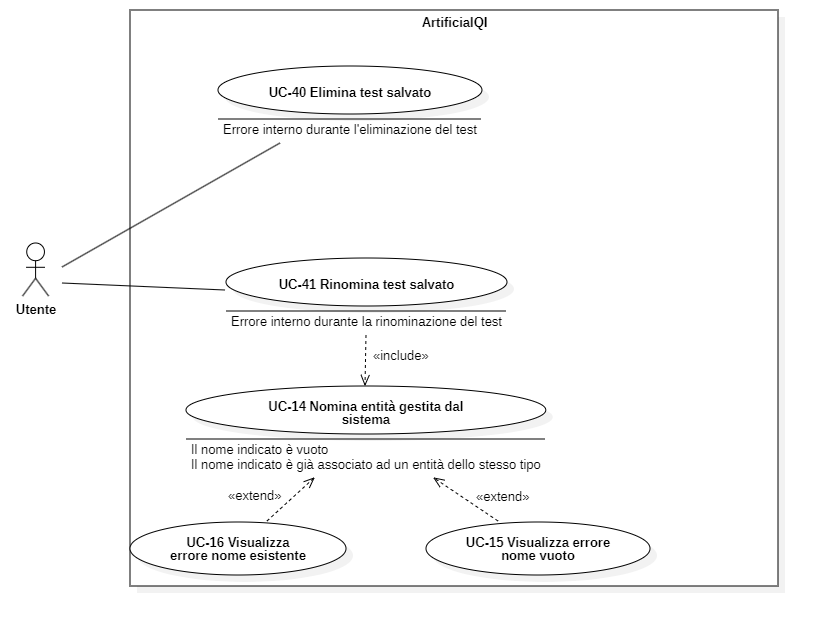
\includegraphics[scale=0.5]{Sezioni/UseCase/Immagini/ModificaTestSalvato.png}
    \caption{Diagramma per la Modifica di un test salvato.}
\end{figure}

\begin{usecase}{UC-40}{Elimina test salvato}
    \label{uc:UC-40}
    
    \req{\hyperref[ru:RUF-1]{RUF-1}}
    
    \pre{
        \item L'utente sta visualizzando i test salvati
        \item Il test da eliminare esiste
    }
    
    \post{
        \item Il test salvato viene eliminato
    }
    
    \actor{
        Utente
    }
    
    \subactors{}
    
    \trigger{L'utente vuole eliminare un test salvato}
    
    \inc{}
    
    \base{}
    
    \scenario{
        \item L'utente richiede di eliminare un test salvato
        \item L'utente conferma l'eliminazione
        \item Il sistema elimina il test 
        \item Il sistema notifica l'utente della corretta eliminazione
    }
    
    \subscenario{
        \item[2.1] L'utente annulla l'eliminazione:
        \begin{itemize}
            \item Il sistema annulla l'operazione
        \end{itemize}
        \item[3.1] Avviene un errore interno durante l'eliminazione del test:
        \begin{itemize}
            \item \hyperref[uc:UC-13]{UC-13}
        \end{itemize}
    }

\end{usecase}

\begin{usecase}{UC-41}{Rinomina test salvato}
    \label{uc:UC-41}
    
    \req{\hyperref[ru:RUF-1]{RUF-1}}
    
    \pre{
        \item L'utente sta visualizzando i test salvati
        \item Il test da rinominare esiste
    }
    
    \post{
        \item Il test salvato viene rinominato
    }
    
    \actor{
        Utente
    }
    
    \subactors{}
    
    \trigger{L'utente vuole rinominare un test salvato}
    
    \inc{\hyperref[uc:UC-14]{UC-14}}
    
    \base{}
    
    \scenario{
        \item L'utente richiede di rinominare un test salvato
        \item Il sistema ottiene il nuovo nome per il test seguendo \hyperref[uc:UC-14]{UC-14}
        \item L'utente conferma la rinominazione
        \item Il sistema rinomina il test
        \item Il sistema notifica l'utente della corretta rinominazione
    }
    
    \subscenario{
        \item[3.1] L'utente annulla la rinominazione:
        \begin{itemize}
            \item Il sistema annulla l'operazione
        \end{itemize}
        \item[4.1] Avviene un errore interno durante la rinominazione del test:
        \begin{itemize}
            \item \hyperref[uc:UC-13]{UC-13}
        \end{itemize}
    }

\end{usecase}

\subsection{Confronto test salvati}

\begin{figure}[H]
    \centering
    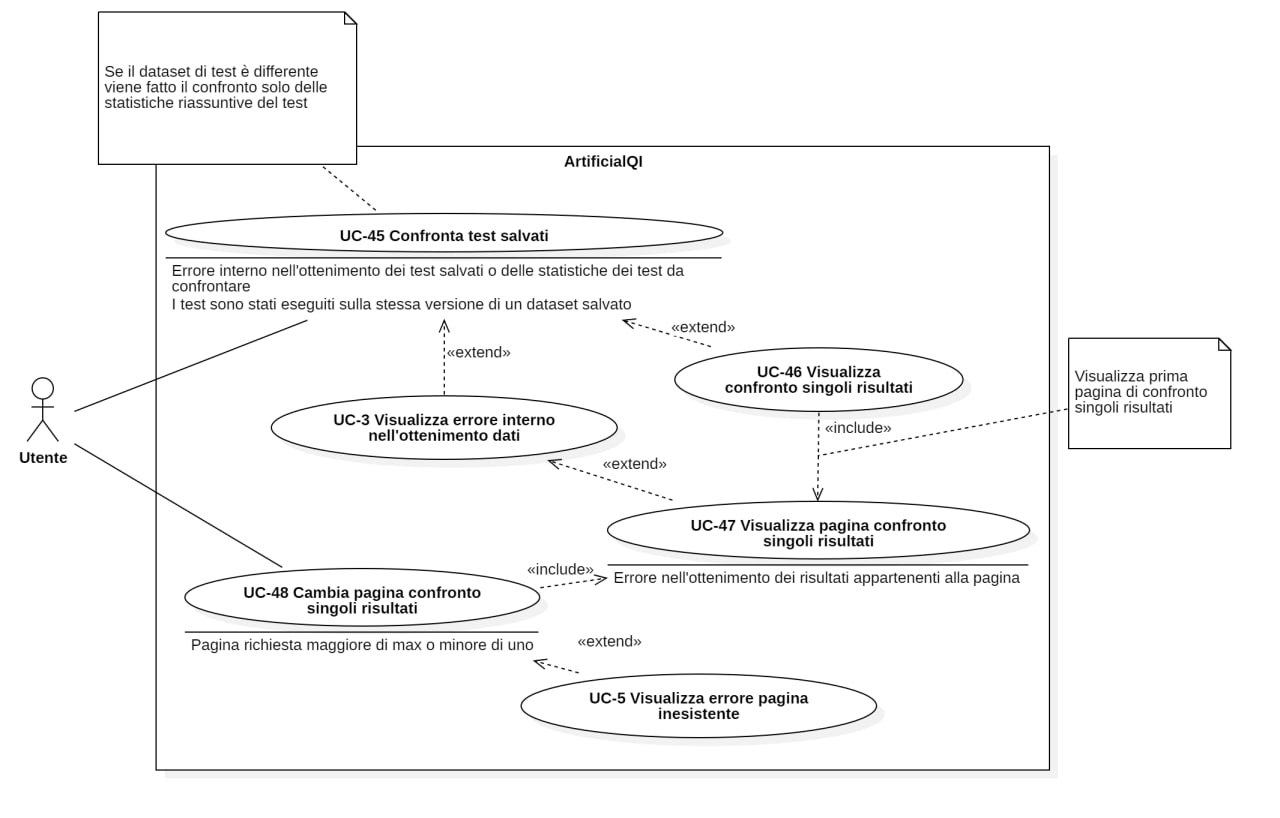
\includegraphics[scale=0.45]{Sezioni/UseCase/Immagini/ConfrontoTest.png}
    \caption{Diagramma per il confronto di test salvati.}
\end{figure}

\begin{usecase}{UC-45}{Confronta test salvati}
    \label{uc:UC-45}
    
    \req{\hyperref[ru:RUF-5]{RUF-5}}
    
    \pre{
        \item L'utente sta visualizzando i risultati del test caricato
        \item Il test caricato condivide il dataset e/o l'LLM utilizzati nel test con almeno un altro test salvato
    }
    
    \post{
        \item L'utente visualizza il confronto tra il test caricato e un test salvato
    }
    
    \actor{
        Utente
    }
    
    \subactors{}
    
    \trigger{L'utente vuole confrontare il test caricato con un test salvato}
    
    \inc{}
    
    \base{}
    
    \scenario{
        \item L'utente richiede l'esecuzione di un confronto con il test caricato
        \item Il sistema richiede la selezione di un test salvato tra quelli che condividono dataset e/o LLM con il test caricato
        \item Il sistema ottiene le statistiche riassuntive del test selezionato
        \item L'utente visualizza i due indici riassuntivi dei test a confronto 
        \item Il sistema verifica che i due test confrontati non siano stati eseguiti sulla stessa versione del dataset
    }
    
    \subscenario{
        \item[2.1]Avviene un errore interno durante l'ottenimento dei test salvati confrontabili con il test caricato:
        \begin{itemize}
            \item \hyperref[uc:UC-3]{UC-3}
        \end{itemize}
        \item[3.1] Avviene un errore interno durante l'ottenimento delle statistiche del test:
        \begin{itemize}
            \item \hyperref[uc:UC-3]{UC-3}
        \end{itemize}
        \item[5.1] I test sono stati eseguiti sulla stessa versione di uno stesso dataset:
        \begin{itemize}
            \item \hyperref[uc:UC-46]{UC-46}
        \end{itemize}
    }

\end{usecase}


\begin{usecase}{UC-46}{Visualizza confronti singoli risultati}
    \label{uc:UC-46}
    
    \req{}
    
    \pre{
        \item I due test coinvolti nel confronto sono stati eseguiti sulla stessa versione dello stesso dataset 
    }
    
    \post{
        \item Vengono visualizzati i confronti dei singoli risultati dei due test
    }
    
    \actor{
        Utente
    }
    
    \subactors{}
    
    \trigger{L'utente ha richiesto il confronto tra due test eseguiti sullo stessa versione dello stesso dataset}
    
    \inc{\hyperref[uc:UC-47]{UC-47}}
    
    \base{}
    
    \scenario{
        \item Il sistema visualizza la prima pagina di risultati seguendo \hyperref[uc:UC-47]{UC-47}
    }
    
    \subscenario{}

\end{usecase}

\begin{usecase}{UC-47}{Visualizza pagina confronto singoli risultati}
    \label{uc:UC-47}
    
    \req{}
    
    \pre{
        \item La pagina da visualizzare esiste
    }
    
    \post{
        \item Vengono visualizzati i confronti dei singoli risultati dei due test appartenenti alla pagina richiesta
    }
    
    \actor{}
    
    \subactors{}
    
    \trigger{Il sistema deve visualizzare una pagina contenente i confronti tra i singoli risultati di due test}
    
    \inc{}
    
    \base{}
    
    \scenario{
        \item Il sistema ottiene i risultati che appartengono alla pagina richiesta
        \item Il sistema mostra il diagramma di dispersione contenente sotto forma di coppie di punti i risultati a confronto che appartengono alla pagina richiesta
        \item Il sistema mostra il confronto tra le coppie di risultati in una lista 
    }
    
    \subscenario{
        \item[1.1] Il sistema riscontra un errore interno durante l'ottenimento dei risultati appartenenti alla pagina richiesta:
        \begin{itemize}
            \item \hyperref[uc:UC-3]{UC-3}
        \end{itemize}
    }

\end{usecase}

\begin{usecase}{UC-48}{Cambia pagina confronto singoli risultati}
    \label{uc:UC-48}
    
    \req{}
    
    \pre{
        \item L'utente sta visualizzando il confronto dei singoli risultati di una coppia di test
    }
    
    \post{
        \item Viene visualizzata la pagina richiesta
    }
    
    \actor{Utente}
    
    \subactors{}
    
    \trigger{L'utente vuole visualizzare una specifica pagina di confronto tra i singoli risultati}
    
    \inc{\hyperref[uc:UC-47]{UC-47}}
    
    \base{}
    
    \scenario{
        \item Il sistema verifica che la pagina sia valida
        \item Viene visualizzata la pagina richiesta seguendo \hyperref[uc:UC-47]{UC-47}
    }
    
    \subscenario{
        \item[2.1] La pagina richiesta non è valida ovvero è inferiore a uno o superiore alla pagina massima:
        \begin{itemize}
            \item \hyperref[uc:UC-2]{UC-2}
        \end{itemize}
    }

\end{usecase}

\subsection{Aggiungi nuovo LLM}

\begin{figure}[H]
    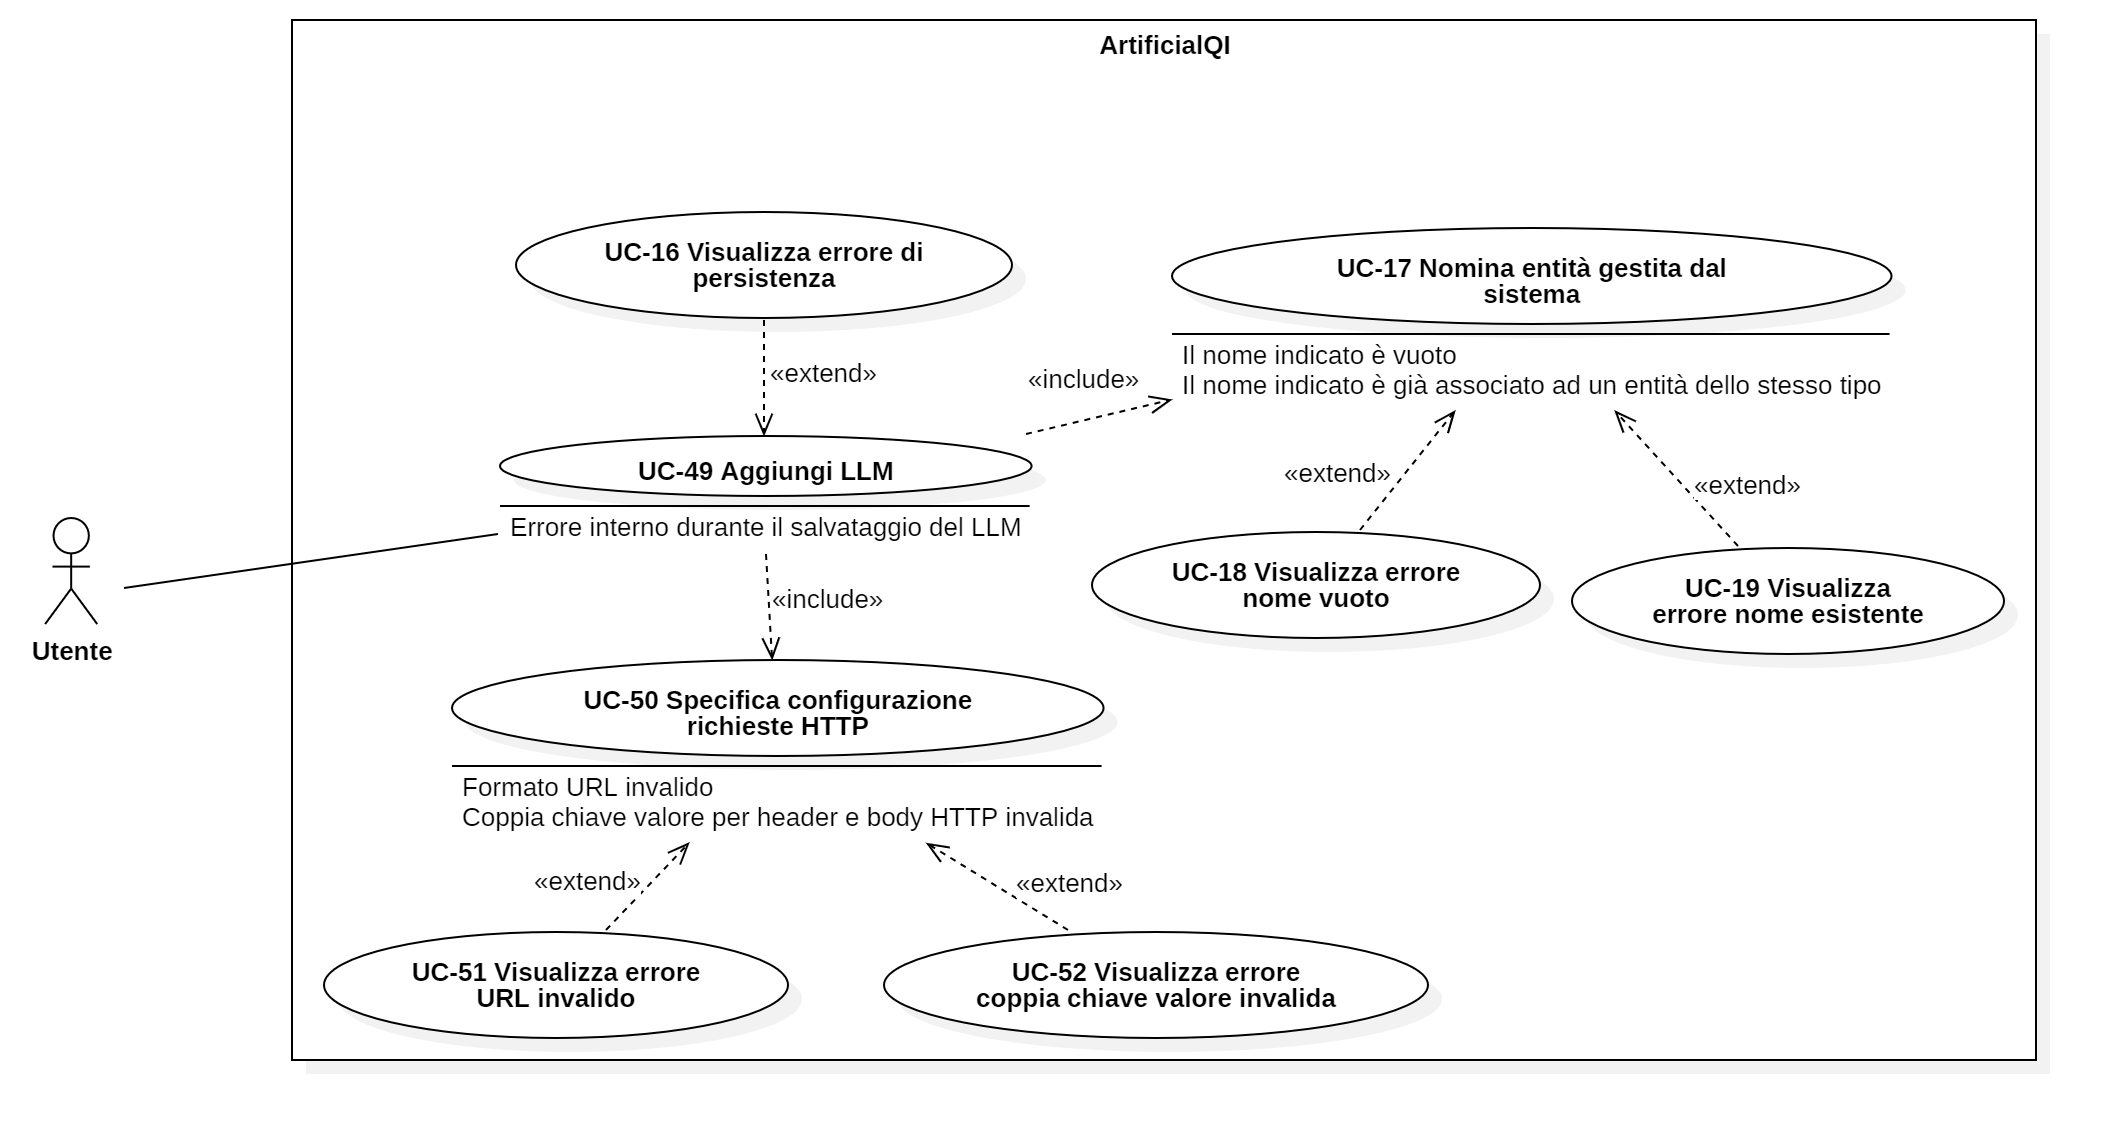
\includegraphics[scale=0.45]{Sezioni/UseCase/Immagini/AggiungiLLM.png}
    \caption{Diagramma aggiungi nuovo LLM.}
\end{figure}

\begin{usecase}{UC-49}{Aggiungi LLM} 
    \label{uc:UC-49}
    
    \req{\hyperref[ru:RUF-6]{RUF-6}} 

    \pre{ 
        \item L'utente sta visualizzando gli LLM salvati \hyperref[uc:UC-55]{UC-55}
    } 
    
    \post{
        \item Viene aggiunto un nuovo LLM nel sistema
    }

    \actor{Utente} 

    \trigger{L'utente vuole aggiungere un nuovo LLM} 

    \inc{\hyperref[uc:UC-17]{UC-17}, \hyperref[uc:UC-50]{UC-50}}

    \base{} 

    \scenario{ 
        \item L'utente richiede di aggiungere un nuovo LLM 
                    
        \item  L'utente specifica la configurazione necessaria per realizzare le chiamate HTTP verso l'LLM seguendo \hyperref[uc:UC-50]{UC-50}
             
        \item Viene richiesta l'assegnazione di un nome per il nuovo LLM seguendo \hyperref[uc:UC-17]{UC-17}

        \item Il sistema salva il nuovo LLM 
    } 

    \subscenario{ 
        \item[4.1] Errore durante il salvataggio dell'LLM:
        \begin{itemize}
            \item \hyperref[uc:UC-16]{UC-16}
        \end{itemize}
    } 
  \end{usecase}
  
  \begin{usecase}{UC-50}{Specifica configurazione richieste HTTP} 
    \label{uc:UC-50}

    \req{} 
    
    \pre{ 
        \item L'utente sta aggiungendo  un nuovo LLM
    } 
    
    \post{ 
        \item Il sistema ottiene la configurazione da utilizzare per le comunicazioni HTTP con l'LLM
    }
    
    \actor{} 
    
    \trigger{
        L'utente deve specificare la configurazione per le richieste HTTP all'LLM
    } 

    \inc{} 
    
    \base{} 

    \scenario{
        \item L'utente specifica l'URL relativo all'LLM
        
        \item L'utente specifica zero o più coppie chiave-valore da utilizzare nell'header HTTP delle richieste verso l'LLM
        
        \item L'utente specifica zero o più coppie chiave-valore da utilizzare nel body delle richieste HTTP verso l'LLM
         
        \item L'utente specifica la chiave da associare alle domande da porre all'LLM
         
        \item L'utente specifica la chiave per estrarre le risposte generate dall'LLM dalla risposta HTTP
    } 
    
    \subscenario{ 
        \item[1.1] Formato dell'URL inserito invalido:
        \begin{itemize}
            \item \hyperref[uc:UC-51]{UC-51}
        \end{itemize}
        \item[2.1] L'utente specifica una coppia chiave-valore invalida:
        \begin{itemize}
            \item \hyperref[uc:UC-52]{UC-52}
        \end{itemize}
        \item[3.1] L'utente specifica una coppia chiave-valore invalida:
        \begin{itemize}
            \item \hyperref[uc:UC-52]{UC-52}
        \end{itemize}
    } 
\end{usecase}

\begin{usecase}{UC-51}{Visualizza errore URL invalido} 
    \label{uc:UC-51}

    \req{} 

    \pre{ 
        \item Il formato dell'ULR è invalido
    } 

    \post{ 
        \item L'utente è a conoscenza che l'URL fornito è in un formato invalido
    }

    \actor{} 

    \trigger{
        Il sistema fallisce la validazione di un URL specificato dall'utente
    } 

    \inc{} 

    \base{} 

    \scenario{
        \item Il sistema mostra un messaggio di errore in cui viene indicato che l'URL è invalido
    } 

    \subscenario{} 
\end{usecase}

\begin{usecase}{UC-52}{Visualizza errore coppia chiave-valore invalida} 
    \label{uc:UC-52}

    \req{} 

    \pre{ 
        \item La chiave o il valore sono vuote o composte da soli spazi
    } 

    \post{ 
        \item L'utente è a conoscenza che la coppia chiave-valore è invalida
    }

    \actor{} 

    \trigger{
        Il sistema fallisce la validazione di una coppia chiave-valore specificata dall'utente
    } 

    \inc{} 

    \base{} 

    \scenario{
        \item Il sistema mostra un messaggio di errore in cui viene indicato che una coppia chiave-valore non può contenere componenti vuoti
    } 

    \subscenario{} 
\end{usecase}


\subsection{Modifica LLM salvato}

\begin{figure}[H]
    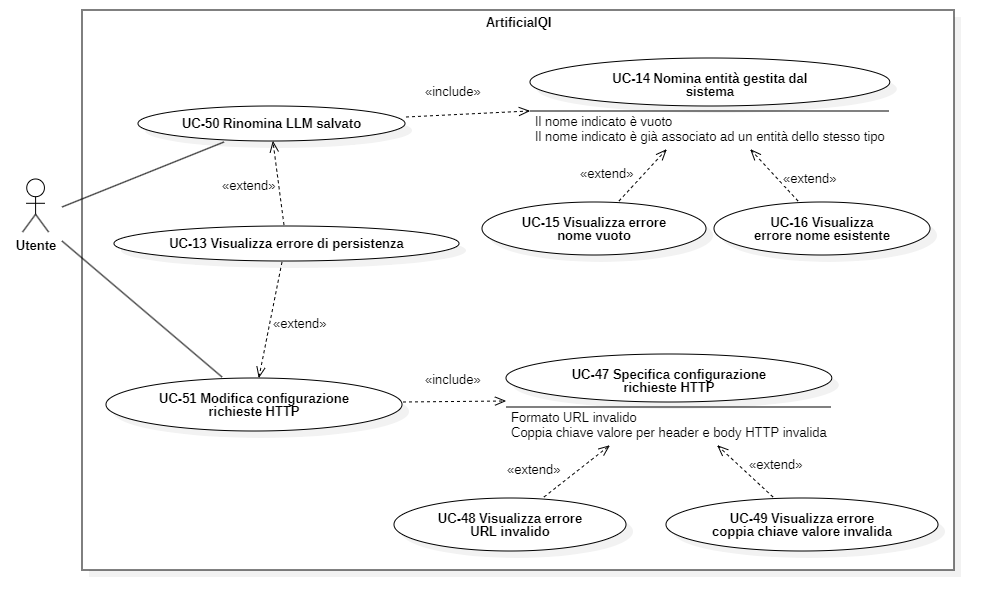
\includegraphics[scale=0.45]{Sezioni/UseCase/Immagini/ModificaLLM.png}
    \caption{Diagramma modifica LLM salvato.}
\end{figure}

\begin{usecase}{UC-53}{Rinomina LLM salvato}
    \label{uc:UC-53}
    
    \req{\hyperref[ru:RUF-6]{RUF-6}} 

    \pre{
        \item L'LLM da rinominare esiste
        \item L'utente sta visualizzando gli LLM salvati \hyperref[uc:UC-55]{UC-55}
    }

    \post{
        \item L'LLM viene rinominato
    }
    
    \actor{Utente}

    \trigger{L'utente vuole rinominare un LLM salvato}

    \inc{\hyperref[uc:UC-17]{UC-17} }

    \base{}

    \scenario{
        \item L'utente richiede la modifica dell'LLM salvato
        \item Il sistema ottiene il nuovo nome per LLM seguendo \hyperref[uc:UC-17]{UC-17}       
        \item Il sistema rinomina l'LLM
        \item Il sistema avvisa l'utente della avvenuta rinominazione
    }

    \subscenario{
        \item[3.1] Avviene un errore interno al sistema durante la rinominazione dell'LLM:
        \begin{itemize}
            \item \hyperref[uc:UC-16]{UC-16}
        \end{itemize}
    }
\end{usecase}

\begin{usecase}{UC-54}{Modifica configurazione richieste HTTP}
    \label{uc:UC-54}
    
    \req{\hyperref[ru:RUF-6]{RUF-6}} 

    \pre{
        \item L'LLM per cui si vuole modificare la configurazione esiste
        \item L'utente sta visualizzando gli LLM salvati \hyperref[uc:UC-55]{UC-55}
    }

    \post{
        \item La configurazione per l'LLM viene modificata
    }
    
    \actor{Utente}

    \trigger{L'utente vuole modificare la configurazione di un LLM salvato}

    \inc{\hyperref[uc:UC-50]{UC-50}}

    \base{}

    \scenario{
        \item L'utente richiede la modifica dell'LLM salvato
        \item Il sistema ottiene la nuova configurazione per il LLM seguendo \hyperref[uc:UC-50]{UC-50}       
        \item Il sistema aggiorna la configurazione dell'LLM
        \item Il sistema avvisa l'utente che la modifica è avvenuta con successo
    }

    \subscenario{
        \item[3.1] Avviene un errore interno al sistema durante la modifica della configurazione:
        \begin{itemize}
            \item \hyperref[uc:UC-16]{UC-16}
        \end{itemize}
    }
\end{usecase}

\subsection{Visualizzazione LLM salvati}

\begin{figure}[H]
    \centering
    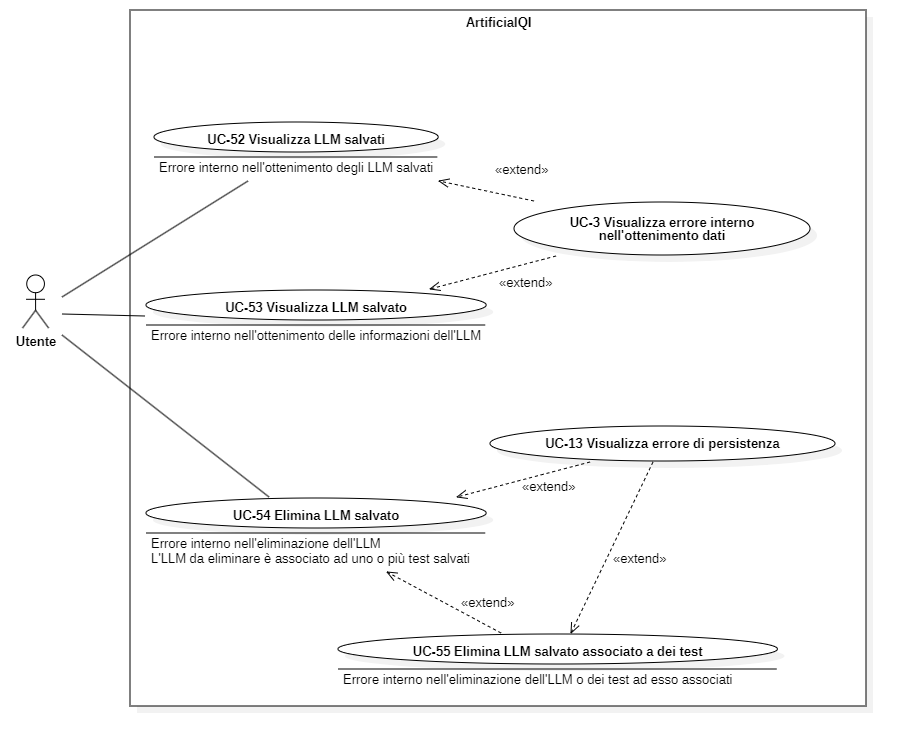
\includegraphics[scale=0.2]{Sezioni/UseCase/Immagini/VisualizzazioneLLMSalvati.png}
    \caption{Diagramma modifica dataset salvati.}
\end{figure}

\begin{usecase}{UC-55}{Visualizza LLM salvati}
    \label{uc:UC-55}
    
    \req{\hyperref[ru:RUF-6]{RUF-6}} 

    \pre{}

    \post{
        \item L'utente visualizza la lista degli LLM salvati
    }
    
    \actor{Utente}

    \trigger{L'utente vuole visualizzare la lista degli LLM salvati}

    \inc{}

    \base{}

    \scenario{
        \item L'utente richiede la visualizzazione degli LLM salvati
        \item Il sistema ottiene l'insieme di LLM salvati
        \item Il sistema verifica la presenza di LLM salvati       
        \item Il sistema mostra gli LLM salvati
    }

    \subscenario{
        \item[2.1] Avviene un errore interno al sistema durante l'ottenimento degli LLM salvati:
        \begin{itemize}
            \item \hyperref[uc:UC-3]{UC-3}
        \end{itemize}
        \item[3.1] Non esistono LLM salvati:
        \begin{itemize}
            \item Il sistema indica all'utente che non esistono ancora LLM salvati
        \end{itemize}
    }
\end{usecase}

\begin{usecase}{UC-56}{Visualizza LLM salvato}
    \label{uc:UC-56}
    
    \req{\hyperref[ru:RUF-6]{RUF-6}} 

    \pre{
        \item L'LLM da visualizzare esiste
        \item L'utente sta visualizzando gli LLM salvati \hyperref[uc:UC-55]{UC-55}
    }

    \post{
        \item L'utente visualizza le informazioni dell'LLM salvato
    }
    
    \actor{Utente}

    \trigger{L'utente vuole visualizzare le informazioni di un LLM salvato}

    \inc{}

    \base{}

    \scenario{
        \item L'utente richiede di visualizzare un LLM salvato
        \item Il sistema ottiene le informazioni sull'LLM       
        \item Il sistema mostra il nome e la configurazione per l'LLM
    }

    \subscenario{
        \item[2.1] Avviene un errore interno al sistema durante l'ottenimento delle informazioni sull'LLM:
        \begin{itemize}
            \item \hyperref[uc:UC-3]{UC-3}
        \end{itemize}
    }
\end{usecase}

\begin{usecase}{UC-57}{Elimina un LLM salvato}
    \label{uc:UC-57}
    
    \req{\hyperref[ru:RUF-6]{RUF-6}} 

    \pre{
        \item L'LLM da eliminare esiste
        \item L'utente sta visualizzando gli LLM salvati \hyperref[uc:UC-55]{UC-55}
    }

    \post{
        \item L'LLM viene eliminato
    }
    
    \actor{Utente}

    \trigger{L'utente vuole eliminare un LLM salvato}

    \inc{}

    \base{}

    \scenario{
        \item L'utente richiede l'eliminazione dell'LLM salvato
        \item Il sistema verifica che l'LLM non sia associato a test salvati 
        \item L'utente conferma l'eliminazione dell'LLM
        \item Il sistema elimina l'LLM
        \item Il sistema avvisa l'utente che l'eliminazione è avvenuta con successo
    }

    \subscenario{
        \item[2.1] L'LLM da eliminare è associato a uno o più test salvati:
        \begin{itemize}
            \item \hyperref[uc:UC-58]{UC-58}
        \end{itemize}
        \item[3.1] L'utente annulla l'eliminazione:
        \begin{itemize}
            \item Il sistema annulla l'operazione
        \end{itemize}
        \item[4.1] Avviene un errore interno al sistema durante l'eliminazione dell'LLM:
        \begin{itemize}
            \item \hyperref[uc:UC-16]{UC-16}
        \end{itemize}
    }
\end{usecase}

\begin{usecase}{UC-58}{Elimina LLM salvato associato a dei test}
    \label{uc:UC-58}
    
    \req{} 

    \pre{
        \item L'LLM da eliminare è associato a uno o  più test salvati
    }

    \post{
        \item L'LLM e i test a esso associati vengono eliminati dal sistema
    }
    
    \actor{}

    \trigger{Il sistema deve eliminare un LLM associato a uno o più test salvati}

    \inc{}

    \base{}

    \scenario{
        \item Il sistema visualizza la lista di test associati all'LLM e avvisa l'utente che verranno eliminati
        \item L'utente conferma l'eliminazione
        \item Il sistema elimina l'LLM 
        \item Il sistema elimina i test associati
        \item Il sistema avvisa l'utente della corretta eliminazione
    }

    \subscenario{
        \item[2.1] L'utente annulla l'operazione di eliminazione:
        \begin{itemize}
            \item Il sistema annulla l'operazione
        \end{itemize} 
        \item[3.1] Avviene un errore interno al sistema durante l'eliminazione dell'LLM:
        \begin{itemize}
            \item \hyperref[uc:UC-16]{UC-16}
        \end{itemize}
        \item[4.1] Avviene un errore interno al sistema durante l'eliminazione dei test associati:
        \begin{itemize}
            \item \hyperref[uc:UC-16]{UC-16}
        \end{itemize}
    }
\end{usecase}